% ---------------------------------------------------------------------
% Das Dokument kompiliert mit pdflatex und ist auf Basis 
% von Koma-Script entstanden. 
%
% Autor des Templates (für Anmerkungen): 
% Michael von Riegen, riegen@informatik.uni-hamburg.de
%
% Einzelne Code-Teile für das Titelblatt sind aus dem Template 
% von Benjamin Kirchheim entnommen.
%
% 25.05.09, Frank Langanke: Vorlage auf aktuelle KOMA-Version aktualisiert
% 26.05.09, Michael von Riegen: Anmerkung --> aktuelles Koma-Script ist nötig!
% 17.10.2016 neues Uni logo
% ---------------------------------------------------------------------
\documentclass[11pt,DIV=15,BCOR=20mm,bibliography=totoc]{scrbook}

% Import von Paketen und Optionen die das gesamte Dokument betreffen
% sind in myPreamble.sty ausgelagert.

\usepackage{myPreamble}

\usepackage[backend=bibtex8,
	style=alphabetic,
	citestyle=alphabetic,
	alldates=edtf]{biblatex}
  
\addbibresource{Bachelorarbeit.bib}  

\usepackage{graphicx}
\usepackage{wrapfig}
\usepackage[format=plain,indention=.3cm,font=it]{caption}
\usepackage{tabularx}

% Arbeitet man nur an einem Kapitel, wird durch folgenden Befehl nur dieses eingebunden.
% Spart manuelles auskommentieren von vielen include-Befehlen;
% hat keine Auswirkung auf input-Befehle
% \includeonly{kapitel1}
   
\begin{document}

%% TITELSEITE
\begin{titlepage}

	% Fehler "destination with the same identifier" unterdrücken...
  \setcounter{page}{-1}

	% Titelseite
	\begin{figure}[h]
		\begin{minipage}[b]{62mm}
			
\includegraphics[width=62mm]{images/unilogo}
		\end{minipage}
		\hspace{4cm}
		\begin{minipage}[b]{59mm}
			
\includegraphics[width=59mm]{images/minlogo}
		\end{minipage}
	\end{figure}

	\vfill
	
	\begin{center}
		% Diplomarbeit 
		\noindent { \huge
			Bachelor Thesis \\
		}
		\vspace{14mm}
		% Titel
		\noindent \textbf{\huge
		  Multitouch Robot Control \\
		}
		\vspace{60mm}	
	\end{center}
	
	\vfill
	
	\noindent \textbf{Merlin Steuer} \\
	\noindent \rule{\textwidth}{0.4mm} 
	\noindent{\textrm{2steuer@informatik.uni-hamburg.de}} \\
	\noindent{\textrm{Studiengang Informatik}} \\
	\noindent{\textrm{Matr.-Nr. 6415125}} \\
	\noindent{\textrm{Fachsemester 10}} \\
	\begin{tabbing}
	\hspace{8em} \=  \kill
	Erstgutachter: \> Dr. Norman Hendrich \\
	Zweitgutachter: \> Dennis Kruppke \\
	~ \\
	Abgabe: 23.04.2018
	\end{tabbing}
	
	% Rückseite der Titelseite mit Zitat
	\newpage 
	\thispagestyle{empty}
	\setcounter{page}{0}

	% wenn man Lust auf ein Zitat hat...
	% ... ansonsten auskommentieren
	~\\ \vfill \noindent 
	Mein Dank gilt all denen, die mich hierbei unterstützt haben -- insbesondere Sven, meinen Eltern und Anna-Lia. Danke.
	\textit{-- Merlin Steuer}
\end{titlepage}



%% VERZEICHNISSE (Inhaltsverzeichnis, Abkürzungen)
% Vorspann einleiten --> Seitennummerierung römisch
\frontmatter

% Inhaltsverzeichnis
\tableofcontents
\cleardoublepage

% Hauptteil einleiten --> Seitennummerierung wieder arabisch
\mainmatter

\chapter{Introduction}

\begin{wrapfigure}{R}{0.2\textwidth}
	\caption{KuKa LWR Arm with Shadow C5 Hand installation\label{fig:armwithhand}}
	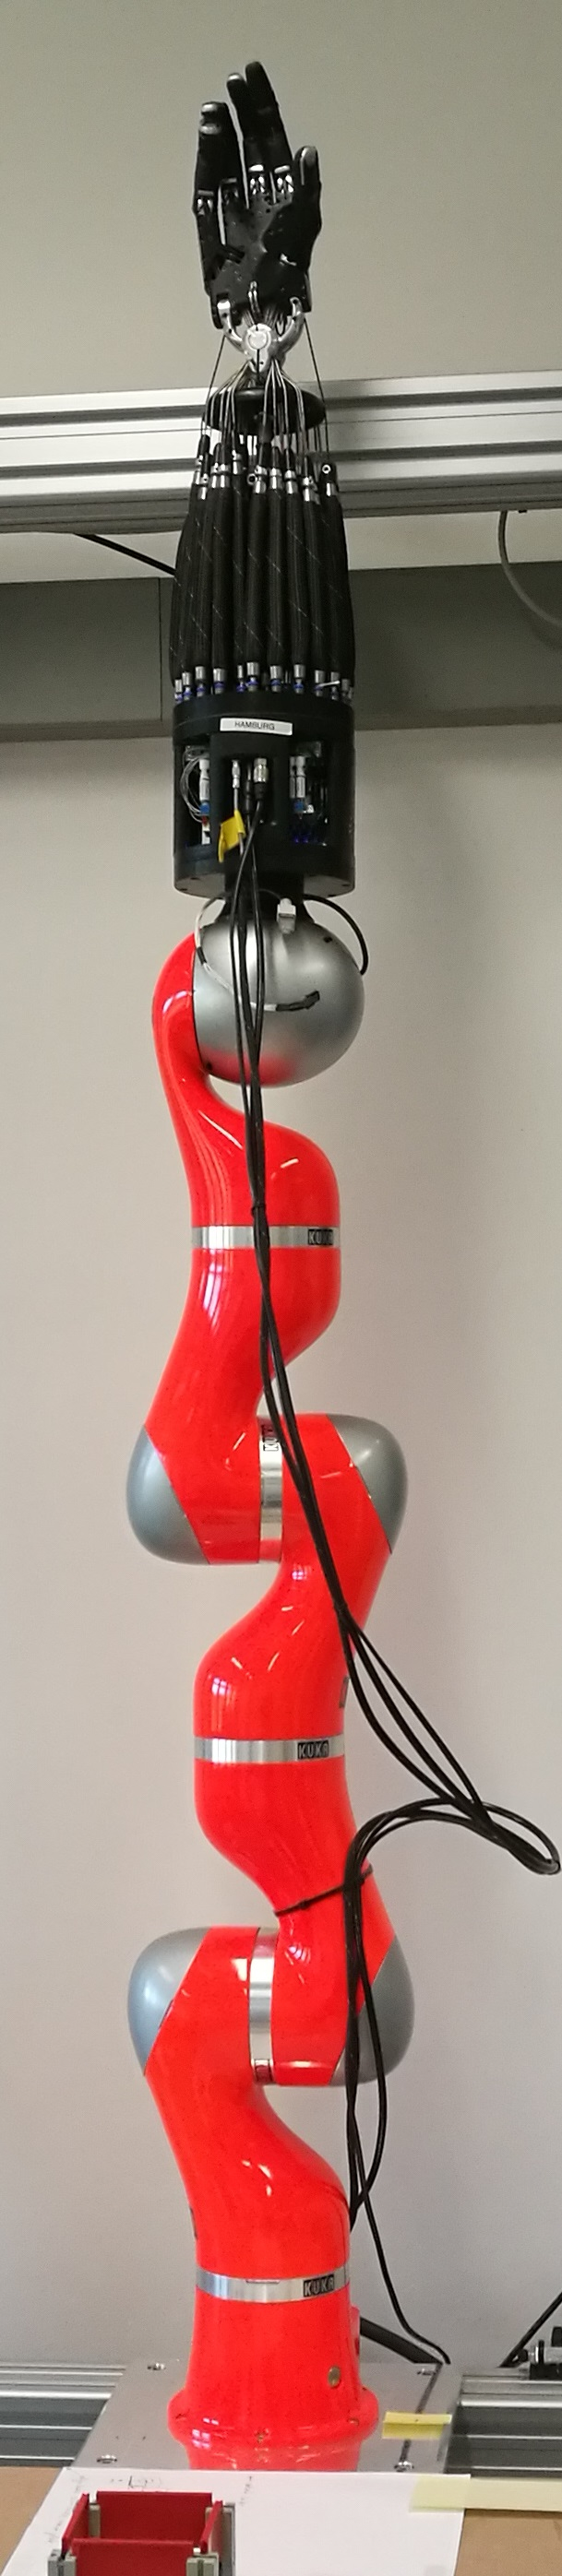
\includegraphics[width=0.2\textwidth]{assets/chpt_intro/lwr_c5hand.jpg}
\end{wrapfigure}

\section{Motivation}

Controlling dexterous robot hands is a big challenge of robotics, but their usage has a variety of obvious advantages: The similarity to a human hand enables it to grasp objects in nearly all positions and poses the real human hand could. Especially for complex manipulation tasks, where a simple robotic grasper with just a pair of pliers is not sufficient, the larger amount of degrees-of-freedom comes into action. Also, users might be able to better plan actions when they are controlling a device similar to their own hands, meaning the main task for them is to use a control interface to execute actions they would otherwise execute with their own hands. Additionally, the robotic hand potentially has more advantages than the human hand, higher degrees-of-freedom, more strength or special fingertips adding more friction and by that enabling grasping of more (e.g. very sleek) different materials. This would give users the ability to perform tasks as they would with their own hands but with less effort or more effective.

\section{Objectives}

Within this thesis, a touch-interface for controlling such robotic hands shall be developed, taking advantage of the multi-touch capabilities of modern mobile tablet computers. The user shall be able to control the position of the robotic hand (using the connected robotic arm) and grasp objects with it. All actions shall be mapped to corresponding multi-touch gestures the user can easily understand and learn.

The hardware used within this bachelor thesis is a \textit{Shadow Dexterous Hand C5/C6} by the Shadow Robot Company. It has five fingers controlled by electrical or pneumatic muscles using 20 degrees-of-freedom\cite{web:robothand:spec}. The hand is connected to a robotic arm (\textit{KUKA Lightweight Robot}) allowing it to also be moved in space (See Figure \ref{fig:armwithhand} for an image of the installation).

As a control device an off-the-shelf android tablet will be used, as these devices have become very widespread and - thanks to this - relatively affordable. With screen sizes of 10 inches and above combined with the capability to record more than 5 independent touch pointers and a number of additional sensors (gyroscope, orientation, ...) and feedback actuators (vibration, sound, ...) they make a good choice for a versatile control device.

Specifically, development during this thesis will take place on a \textit{Samsung Galaxy Tab S3}. It has a screen size of 9.7 inches\cite{samsung:galaxytabs3} with a resolution of 2048x1536 pixels accompanied by a 2.15GHz Quad-Core processor. These properties give it the ability to also perform some calculation-heavy tasks locally, giving the overall application a better performance. The used Android tablet runs Android 7.0. One goal of this thesis is to make the control application available to a broad variety of devices. Because of this, the application shall run on Android down to Version 4.3 and up to the current 7.0.

A native Android application will be developed and run directly on the tablet. As a programming language Java is chosen, as it is the language natively used on Android. Multiple approaches to the problem will be implemented to give users and researchers the ability to test and evaluate multiple methods against their usability, effectiveness and user-friendliness.

\section{Outline}

In Chapter \ref{chap:basics} a brief overview over the technology used during the development of this thesis will be described and explained to give the reader a profound basis of knowledge to understand the processes and decisions described later. Chapter \ref{chap:concepts} depicts the concepts and architectural design process decisions made for later development. The implementation is then described in detail within Chapter \ref{chap:implementation}. Proposals for user studies and usability evaluations are then made in Chapter \ref{chap:eval}, as they are not part of this thesis.

\chapter{Related work}

A lot of research is and was done in the field of remote-controlling robots with generic devices. This is most probably the case due to them being ubiquitous and well-known by common users. This is important as more and more robots have entered the personal living spaces of users during the last 2 decades\cite{Forlizzi2006} which have to be controlled by untrained persons with the least possible amount of learning. This leads to the need of very easily understandable user interfaces and a small amount of complexity in the possible controls. 

One approach to reduce complexity in controlling a robot with a high amount of degrees-of-freedom (DOF) is described in \cite{Bernardino2013}. The researchers conducted a principal component analysis (PCA) on different grasping hand poses. The calculated components can then be used to control a device with e.g. 22 DOF by just 2-3 parameters. As this thesis is partly based on this approach and the given research, more explanation can be found in Chapter \ref{chap:concepts}. Apart from this analytical approach another part of this thesis is based on \cite{conf:humanoids:TohHLBZP12} where researchers developed a method to directly map finger positions on a tablet computer to those on a robotic hand. These are the two main approaches examined in this thesis.

Other ideas to teleoperate robots with generic devices are numerous. A similar approach is to control a mobile robot using an android device by tilting it\cite{Akupati2017}. The idea here is to simulate a steering wheel of a car to move a car-like robot. 

As the fields of virtual reality (VR) and augmented reality (AR) gain more and more attention, different approaches to remotely control robots assisted by such VR systems come up. Hashimoto et al. developed a software called TouchMe, displaying a video image of a robot, allowing to directly alter a robot model perfectly laid over the video image using simple drag and drop actions on a touchscreen\cite{Hashimoto2013}. Krupke et al. took the approach one step further by displaying the virtual environment on a head mounted device (HMD, also referred as \textit{VR glasses}). The HMD displays a virtual representation of the manipulated device, allowing the controller to look at the scene from arbitrary angles. Fine control was implemented by putting the controller's hand into a virtual sphere and recording hand movement while mapping it to movements of the controlled robot.


\chapter{Basics}
\label{chap:basics}
\section{ROS - The Robot Operating System}

The \textit{Robot Operating System} (ROS) is an open-source software framework providing a robust communication layer for distributed robot computing\cite{ros:intro}. Despite the name it is not an operating system in the traditional manner, as it does not provide or implement any processing, scheduling or data access functionality. It is a set of programs and libraries enabling developers to develop so-called \textit{nodes} that communicate with each other using the \textit{Publish-Subscribe-Pattern}.
This pattern allows multiple loosely-coupled nodes (applications) to exchange messages. This design allows a greater reuse of code since software for robots is written very modular\cite{Eugster2003}. For example, on a robot with a laser scanner and a motor, one node would decode the laser scanner data, publish the results to a specific topic which is subscribed by a controller node, that processes the data and then publishes motor control messages to another topic, which is again subscribed by the motor controller node. All nodes do not have to know each other. This makes it very easy to reuse the code for either the laser scanner or the motor driver node in other configurations (like multiple different robots) or exchange the controller node that processes the data. Using wireless connections, it is also possible to move specific processing tasks to external (\textit{off-board}) nodes. This comes in handy for example in terms of image processing, which is a task that usually overloads small on-board processing units built into robots.

The communication is organized by a program called \textit{ROS Core}. All nodes connect to this Core and tell it what they'd like to do (e.g. subscribing to topics, publishing to topics etc.). To reduce communication overhead, the actual data exchange is then done in a peer-to-peer manner, meaning the nodes directly exchange data with each other over TCP/IP. This also means that all nodes have to be able to reach each other, which might lead to problems when running ROS in bigger networks.

Sometimes, the publish-subscribe-pattern (and its inherent asynchrony) are not sufficient, as some calculations, which might be too heavy to be executed locally, might still have to be done synchronously. For this case, ROS introduces so-called \textit{services}. These are basically function calls that are offered by a node which may then be called by any other node over the network. These calls are executed synchronously and directly return a result.

Nodes have names seperated in so-called \textit{name spaces}. an example node name can look like in Listing \ref{code:ros:nodename}.
\begin{lstlisting}[caption={An example ROS node name},label=code:ros:nodename]
/robot/hand/controller
\end{lstlisting}


where \textit{/robot/hand} is the name space and \textit{controller} the node name. Topics and services do also have a specific name including a name space. This addressing scheme allows it to have multiple equally-called nodes or topics (e.g. for multiple sensors of the same type) by just putting them into different name spaces but preserving there names.

Numerous implementations of the ROS client libraries are available, the most common ones are developed and used in C/C++ and Python\cite{ros:client_libraries}. For developing a ROS-enabled Android application, an implementation of the ROS client library in Java is chosen. 

\subsection{Rosjava / Rosandroid}

There is an implementation of the ROS client library published on GitHub\footnote{\url{https://github.com/rosjava/rosjava_core}}. It includes support for all needed communication structures within ROS as well as the most common message types exchanged with ROS nodes. \textit{rosjava} is specifically designed to develop ROS-enabled Android applications and is originally developed by Google\cite{ros:rosjava:readme}.

The package \textit{rosandroid}\footnote{\url{https://github.com/rosjava/android_core}} is an extension of \textit{rosjava}. It offers functionalities to easily include ROS support into an Android application by offering readily usable \textit{Activities}\footnote{Activities are offering the user interface in Android applications} to connect the application to a ROS core or start an independent core within the application itself. It also includes some basic user controls like a joystick control which we will not make use of within this thesis.

\textit{rosandroid} is designed for the newest versions of Android, which leads to the fact that a small change has to be made in the code to make it compatible with older versions of Android, too. These changes are described in Chapter \ref{impl:compiling_rosandroid}.

\subsection{Using Services in Rosjava}
\label{sec:using_services}
The implementation of how to consume (i.e.~call) services is a little different in rosjava than it is in roscpp\footnote{roscpp is the C++ implementation of ROS}, which is why the main differences will be briefly be elaborated here. To call services, special ROS messages are exchanged. These so-called \textit{service message types} consist of a request and a response part. While in C++ one object containing both the request and the response is passed to the \textit{service client} which then fills out the response part\cite{ros:serviceclient}, in other implementations like \textit{rospy} or \textit{rosjava} these messages are separated.

To create a \textit{service client} in rosjava, an instance of 

\begin{lstlisting}[numbers=none]
org.ros.node.service.ServiceClient
\end{lstlisting}

is created within the \textit{onStart} callback of the node, passing the name of the service node and the service message types. Listing \ref{lst:rosservice} demonstrates how such a start-up routine could look like.

\begin{lstlisting}[caption={Example on how to connect to a ROS service in rosjava},label=lst:rosservice]
@Override
public void onStart(ConnectedNode connectedNode) {
// ....
	try {
		ikService = connectedNode.newServiceClient("/bio_ik/get_bio_ik", bio_ik_msgs.GetIK._TYPE);
	} catch (ServiceNotFoundException e) {
		ikService = null;
		e.printStackTrace();
	}	
// ....
}
\end{lstlisting}

In \textit{rosjava} no such method like \textit{Ros::waitForService()} (in C++) is present\footnote{Albeit requested by multiple users, like in \url{https://github.com/rosjava/rosjava_core/issues/105}}. As rosjava is designed in a way that one application can implement multiple ROS nodes, a blocking call to the above method would cause the rest of the application to stop working, which is probably the reason why the developers of rosjava have decided not to implement it. In rosandroid applications, a blocking wait-call would cast the user interface unresponsive and thus unusable. Developers have to make sure that, in the time a node starts, the service it wants to consume is already registered with the \textit{ROS Master}.

Once the \textit{ServiceClient} is created it can be used by creating a new request message. Confusingly, request and response message types are separated in service calls, while the combined message type is passed to the \textit{newServiceClient} method. An example service call is presented in Listing \ref{lst:servicecall}.

\begin{lstlisting}[caption={An example rosjava service call}, label=lst:servicecall]
bio_ik_msgs.GetIKRequest greq = ikService.newMessage();
IKRequest req = greq.getIkRequest();
// ... fill in the request parameters into the req object ...

ikService.call(greq, new ServiceResponseListener<GetIKResponse> {
	@Override
	public void onSuccess(GetIKResponse getikResponse) {
		// Handle service response
	}
	
	@Override
	public void onFailure(RemoteException e) {
		// Handle service error
	}
});
\end{lstlisting}

Two things are important to note here. Firstly, the messages exchanged are not \textit{IKRequest} and \textit{IKResponse} as the names would suggest, but \textit{GetIKResponse} and \textit{GetIKRequest}, which are created automatically by the rosjava message generator. The latter service messages then contain the corresponding former message types. This is one main difference in calling ROS services between Java and C++ implementations. Secondly, the service response is processed non-blocking, meaning it is asynchronously passed to the listener object implementing  the 
\begin{lstlisting}[numbers=none]
org.ros.node.service.ServiceResponseListener
\end{lstlisting}
interface. Busy-waiting service calls are not implemented in rosjava, most probably for the same reasons that busy-waiting for services to come up have not been implemented. This asynchrony is the second main difference developers accustomed to \textit{roscpp} have to get used to when switching over to \textit{rosjava}.

\section{The Shadow C5 Robotic Hand}
\label{sec:shadowhand}

\begin{wrapfigure}[13]{R}{0.35\linewidth}
	\vspace{-2.2em}
	\caption{The Shadow C5 hand}
	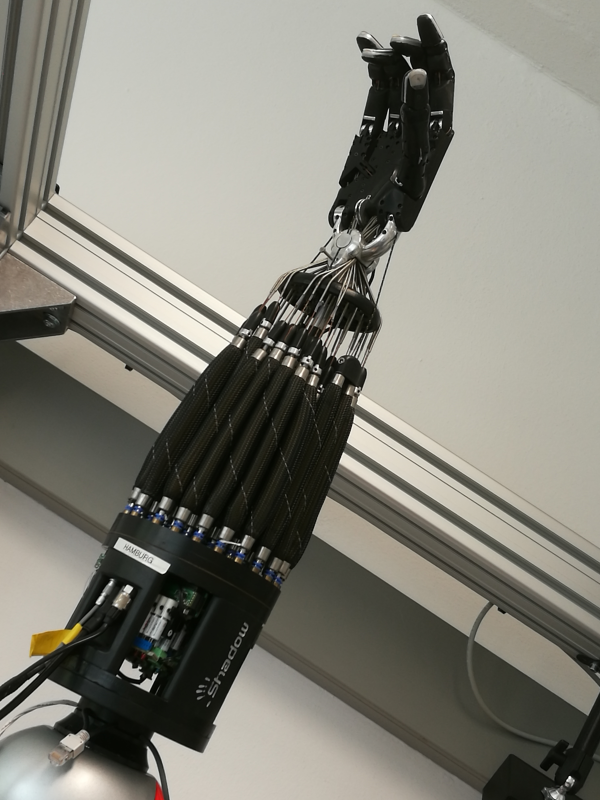
\includegraphics[width=\linewidth]{assets/chpt_basics/hand.png}
\end{wrapfigure}

The \textit{Shadow C5 Robotic Hand} was developed by the \textit{Shadow Company}. It is designed to be as similar to a human hand as possible\cite{web:robothand:spec} in terms of force output, movement speed and movement sensitivity. It has 24 degrees-of-freedom, all controlled by 48 pneumatic muscles. These muscles, when pressurized, contract a little, applying force to the elements of the mechanical hand over imitated tendons. The developers tried to design the product as close to the average human forearm as they could. It weighs about 4kg and has a maximum movement speed of about half the speed at the joints a human could reach. The pneumatic muscles work with a pressure of 3.5 bar and having a maximum flow of 24 litres per minute, resulting in the need of a relatively powerful air compressor and air pipe system installed near the hand. Joint angles of all joints (controllable as well as non-controllable) are measured by hall-sensors at an accuracy of 0.2 degrees.
A similar robotic hand powered by electrical motors instead of pneumatic muscles is also present at the TAMS group at the University of Hamburg. This thesis will, however, mainly work with the pneumatic powered hand. 
\newpage
\subsection{Integration into ROS}

\begin{wrapfigure}{L}{0.4\textwidth}
	\vspace{-2.2em}
	\caption{\label{fig:hand:ros_integration}Schematic overview to the integration of the hand into a ROS environment}
	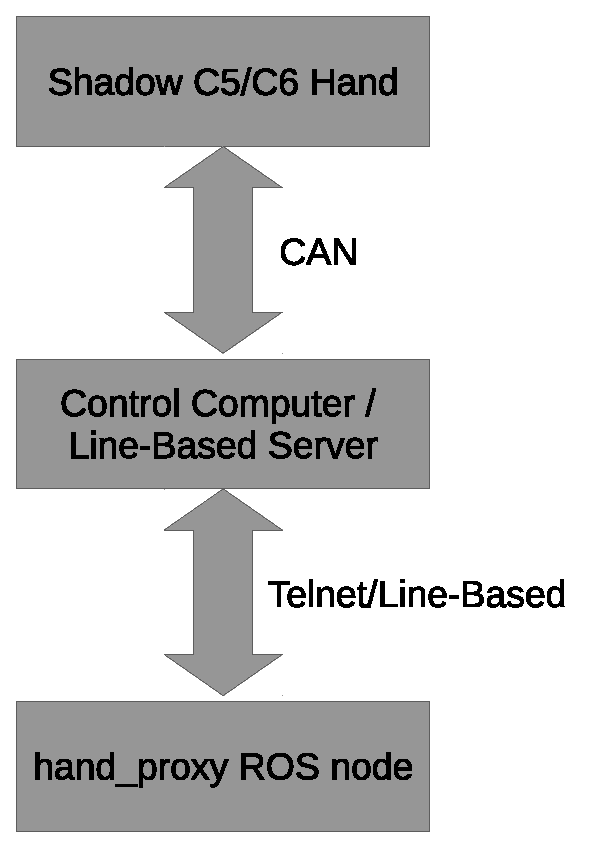
\includegraphics[width=0.4\textwidth]{assets/chpt_basics/hand/ros_integration.eps}
\end{wrapfigure}

The Shadow Robotic Hand possesses by default a CAN-Bus (Controller Area Network) interface over which it is controlled\cite{web:robothand:spec}. The CAN protocol has been implemented using a parallel port on a distinct machine next to the robotic hand. To have the ability to communicate with the hand over network, a server application has been implemented by members of the TAMS group at University of Hamburg. 
Multiple applications have been developed to control the robotic hand without the integration of ROS. To make use of the features and advantages of a ROS environment, a ROS proxy was implemented. It basically listens to a ROS topic where it receives joint target states and publishes to another ROS topic where it sends the current measured joint angles to. The ROS hand proxy node communicates with the hand server over the line-based protocol and converts all data it receives for the corresponding other side. This set-up makes it easy to integrate the Shadow C6 hand into a ROS environment. See Figure \ref{fig:hand:ros_integration} for a schematic overview of how the robotic hand is integrated into ROS.

\begin{table}
	\caption{\label{tab:rosmsg:topics}Topics used to send and receive joint states}
	\begin{tabularx}{\linewidth}{|c|X|}
		\hline
		\textbf{/hand/joint\_states} & The ROS hand proxy publishes the current measured joint states it received from the hand server to this topic \\
		\hline
		\textbf{/hand/joint\_goals} & The ROS hand proxy receives packages containing joint states sent to this topic and passes it on to the hand server, causing the hand to try to reach the sent joint angles. \\
		\hline
	\end{tabularx}
\end{table}

The two important topics used throughout this thesis are denoted in Table \ref{tab:rosmsg:topics}. The message type used for both of these topics is \textit{sensor\_msgs/JointState}. These messages consist of the data fields denoted in Table \ref{tab:rosmsg:contents}. A few things are important to be considered while using the data contained in these messages. First, how the data is interpreted is application-specific. While the data fields contain arbitrary data it is important to know that the set-up used in this thesis only has rotating joints, meaning the data in the position field is in radians. For other types of joints (e.g. linear joints) this could possibly deviate. Second is, the order of elements is not important, however it is very important to maintain corresponding elements' positions at the same index within the \textit{names} and the \textit{position} fields. This means that e.g. the position for joint \textit{THJ1} must have the same index in the \textit{position} field as the string \textit{THJ1} in the \textit{names} field. Finally it is important to note that the \textit{effort} and \textit{velocity} fields are currently not used for the set-up. When these rules are followed it is easy to send joint states to the robot and observe its movement.

\begin{table}
	\caption{\label{tab:rosmsg:contents}Contents of the  \mbox{sensor\_msgs/JointState} message type}
	
	\begin{tabularx}{\linewidth}{|c|X|}
		\hline
		\textbf{Field} & \textbf{Description} \\
		\hline
		header & Header information including a time-stamp of when the message was sent and a sequence number of the message \\
		\hline
		names & Array of strings containing the joint names the other fields contain information about \\
		\hline
		position & Array of floats containing the position of each joint \\
		\hline
		velocity & Array of floats containing information about the velocity at which each joint is currently or shall be moving \\
		\hline
		effort & Array of floats containing information about with how much efford (e.g. force) a joint shall be or is moved \\
		\hline
	\end{tabularx}
\end{table}

\section{The Kuka Lightweight Robot Arm}

\begin{wrapfigure}[8]{R}{0.35\linewidth}
	\vspace{-2.2em}
	\caption{The Kuka LWR robot arm}
	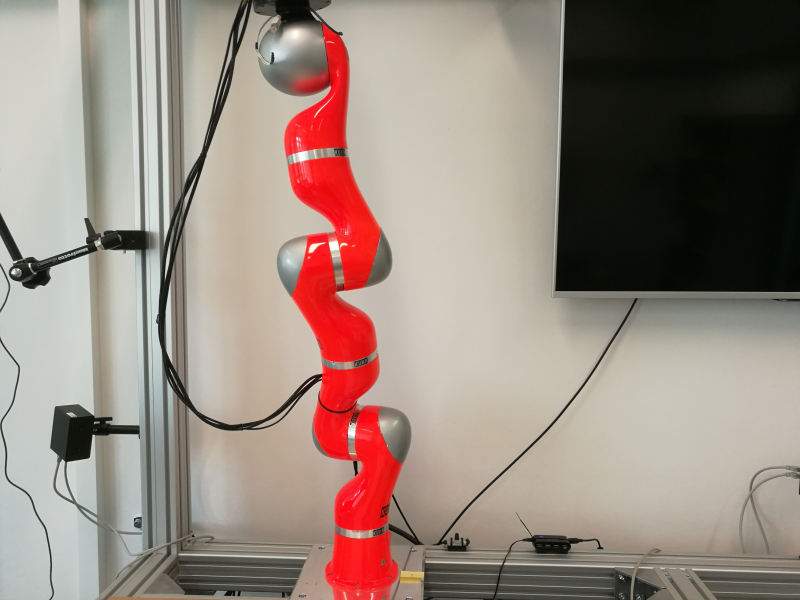
\includegraphics[width=\linewidth]{assets/chpt_basics/arm.png}
\end{wrapfigure}

The robotic arm used in the set-up is a \textit{Lightweight Robot 4+} by the German company \textit{KUKA Roboter Gmbh}. It has 7 degrees-of-freedom, allowing it to operate in a space as big as approximately $1.8m^3$\cite{Lwr2010}. All joints can be used in ranges of $\pm 170$ or $\pm 120$ degrees. The robot is controlled by a dedicated computer supplied with it. Connected to the computer is an external control interface, which allows basic operations of the robot.

\subsection{Integration into ROS}

To control the robot using ROS a special application has to be launched on the control computer of the robot. This application is called \textit{FRI} (\textit{Fast Research Interface}) and is supplied by the KUKA company\cite{Fri2010}. When this was successful, a special ROS node has to be started on another computer within the same network. This node is called \textit{ros\_fri}. Then messages can be sent to the robot by publishing messages of the type \textit{ros\_fri\_msgs/RMLPositionInputParameters} to the topic:
\begin{lstlisting}[numbers=none]
/lwr/jointPositionGoal
\end{lstlisting}

The contents of the message type are described in Table \ref{tab:frimsg}. When such a message is received by the FRI application the robot will immediately start to move to the given position. The arrays in the message all have to have the correct number of entries (i.e.~7, one for each joint). If no value shall be set, a zero value has to be inserted anyway.


\begin{table}
	\caption{\label{tab:frimsg}Contents of the RMLPositionInputParameters message type}
	\begin{tabularx}{\linewidth}{|l|X|}
		\hline
		\textbf{Field} & \textbf{Description} \\
		\hline
		double[] target\_position\_vector & Desired target positions of all joints in radians. \\
		\hline
		double[] target\_velocity\_vector & Desired movement velocities of all joints. \\
		\hline
		double[] max\_acceleration\_vector & Maximum allowed acceleration for all joints. \\
		\hline
		double[] max\_velocity\_vector & Maximum movement velocity allowed for each joint. \\
		\hline
	\end{tabularx}
\end{table}

\section{Inverse Kinematics}

Inverse kinematics is one of the challenging fields in many applications like robotics or computer animations\cite{Starke2017}. To understand what inverse kinematics is, it is important to look at a robot (or e.g. animated figures in video games) from two different points of view. The normal viewer would describe the position and pose of a robot or effector in his own coordinate system, usually in Cartesian coordinates. This position can be described as an $n$-dimensional vector $X$. To describe movement of the robot, the viewer would then tell a difference between the new and the old position vectors $X_{new}-X=\Delta X$. A robot, however, often cannot move in Cartesian space, as its kinematic chain (i.e.~the parts of the robot connected by rotational or translational joints) can have $m$ degrees-of-freedom (DOF) with $m > n$. The position in the so-called \textit{joint-space} is referred to as $\theta$. To control such a robot with a high number of DOF, the controller has to be aware of the current position of the robot in Cartesian space $X$, the desired position change $\Delta X$ and the change in joint-space $\Delta \theta$ that has to be applied to the current position in joint space $\theta$. $\theta$ is known by the current state of the robot, finding $X$ is done by applying \textit{forward-kinematics} to $\theta$:
\begin{equation*}
	X = f(\theta)
\end{equation*}

Forward kinematics usually is a straight-forward process of beginning at the base of the robot and iterating through all joints up to the \textit{end-effector} to find its position. The inverse kinematics to find the corresponding position in joint-space to reach the desired position in Cartesian space
\begin{equation*}
\theta = f^{-1}(X)
\end{equation*}
however is not as easy as the forward kinematics as with rising numbers of DOF no analytical solution is possible and multiple (up to an infinite number) valid joint-positions can exist - or even none at all\cite{DextquotesingleSouza}.

Many approaches to this problem have come up during the years. \citeauthor{andreasaristidou2009inverse} give a good overview over the existing methods in their technical report\cite{DextquotesingleSouza}.

\begin{figure}
	\caption{Forward and inverse kinematics\label{fig:basics:kinematics}}
	\begin{center}
		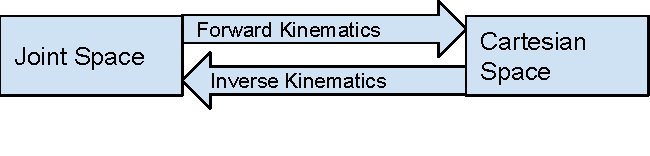
\includegraphics[width=0.6\textwidth]{assets/chpt_basics/Kinematics.pdf}
	\end{center}
\end{figure}

\subsection{BioIK}
\label{sec:bioik}
BioIK is the name of a newly developed algorithm for inverse kinematics at the TAMS research group at the University of Hamburg\cite{Starke2017}. BioIK is a multi-goal evolutionary algorithm. This means in particular, that it accepts goals for multiple end-effectors in a kinematic chain whereas most other algorithms only accept one goal for one end-effector. This makes the algorithm especially suitable for highly articulated robots and models like humanoids\cite{Starkea2017}. Being an evolutionary algorithm means that solutions are created using predecessors and applying random mutation to a solution. Solutions of the algorithm are then classified by a fitness function, while good solutions remain within the so-called genom and bad solutions are not used for further evolutions\cite{Ruppel17} - similar to the so-called and name giving real world evolution. Within this thesis BioIK is used to calculate joint angles for given robot poses. The big advantage of BioIK is that it accepts multiple goals, i.e.~one goal for every fingertip, and calculates corresponding joint positions based on the given goals.

\subsubsection{Integration into ROS}
Philipp Ruppel integrated BioIK into ROS during his Master Thesis\cite{Ruppel17}. He integrated the BioIK solver into \textit{MoveIt!}, which is a motion planning framework integrated into ROS\cite{Coleman15}. Using \textit{MoveIt!} it is possible to plan motions and poses of robots from just calculating a pose of a robot to plan full motion trajectories from one pose to another while avoiding obstacles and collisions.

In addition to the functionality directly calling \textit{MoveIt!} interfaces from C++ a ROS service was implemented to get IK solutions from BioIK over a ROS service from arbitrary nodes - especially from non-C++ nodes like ones written in Java (rosjava, rosandroid) or Python (rospy)\footnote{The implementation of the ROS BioIK Service can be found at \url{https://gogs.crossmodal-learning.org/philipp.ruppel/bio_ik_service}}. 
Having this BioIK ROS service available makes it relatively easy to get IK solutions within nodes separated from \textit{MoveIt!} which is why it will be used within this thesis to request joint positions for given robot poses within the developed Android application. The process of integrating the service into the application (i.e.~requesting joint angles for given robot poses) is described in Chapter \ref{sec:robotarm:ctrl}.

\chapter{Implementation}
\label{chap:implementation}
\section{Preparations}
\subsection{Setting up a virtual machine}

For all developments within this thesis a virtual machine was used. This makes it easy to reproduce the environment within the labs at the TKRN group as well as having a portable development solution isolated from the rest of the computer's operating system. As the ROS version called \textit{Kinetic} is widely used within the set-ups around the robot, I will also develop the application using this version. This reduces the risk of incompatibility issues during development. ROS \textit{Kinetic} is available as packages for Ubuntu up to version 16.04\cite{ros:install}, which is why we install this version of Ubuntu within a new virtual machine. Enough virtual hard disk space and memory is assigned to the virtual machine (200GB HDD, 8 GB RAM) as well as 4 processing cores. This set-up should be sufficient for all purposes during this thesis. 

If the virtual machine shall run ROS nodes which have to be accessible by ROS nodes outside the machine itself (i.e. the Android tablet running the control application) the network interface of the virtual machine should be configured as a bridged network connection. This lets the network's DHCP (if present) assign the virtual machine its own IP address reachable from the network. However, this was not possible within the university's network, as Oracle VirtualBox was not able to create a working bridged network adapter using the computer's Wi-Fi connection. During development within the lab another computer directly connected to the university network was used to run \textit{roscore}.

\subsection{Setting up ROS}

\subsubsection{Installing ROS}

Setting up ROS \textit{Kinetic} within a fresh Ubuntu 16.04 installation is fairly simple. First, the ROS apt\footnote{Aptitude is the package management system for Debian-based Linux distributions like Ubuntu}-repository has to be added to the packages sources file and the corresponding key has to be added to the key storage to enable downloading the packages. Once this is done, the package \textit{ros-kinetic-desktop-full} can be installed which will download and install all available packages for ROS \textit{Kinetic}.

The commands to install ROS are denoted in Listing \ref{lst:ros:install}. After these commands have been executed in a terminal window ROS is readily installed.

\begin{minipage}{\linewidth}
	\begin{lstlisting}[caption={Commands for installing ROS\cite{ros:install}},label={lst:ros:install}]
	sudo sh -c 'echo "deb http://packages.ros.org/ros/ubuntu $(lsb_release -sc) main" > /etc/apt/sources.list.d/ros-latest.list'
	sudo apt-key adv --keyserver hkp://ha.pool.sks-keyservers.net:80 --recv-key 421C365BD9FF1F717815A3895523BAEEB01FA116
	sudo apt-get update
	sudo apt-get install ros-kinetic-desktop-full
	\end{lstlisting}
\end{minipage}

ROS is by default installed to \textit{/opt/ros/kinetic/}. To make use of all available command line tools provided by ROS it is important to load the file \textit{/opt/ros/kinetic/setup.bash} into the currently open (bash)-command-prompt. This is either temporarily done by issuing

\begin{lstlisting}[caption={Temporarily loading the ROS environment into bash}]
source /opt/ros/kinetic/setup.bash
\end{lstlisting}

or permanently by adding this line to the file \textit{$\sim$/.bashrc} by executing the following command:

\begin{lstlisting}[caption={Permamently installing the ROS environment into bash}]
echo "source /opt/ros/kinetic/setup.bash" >> ~/.bashrc
source ~/.bashrc
\end{lstlisting}

When this is done, ROS is completely set up on the development machine.

\subsubsection[Setting up catkin]{Setting up a catkin workspace\cite{ros:install:catkin}} 

\textit{Catkin\footnote{\url{http://wiki.ros.org/catkin}}} is a build system and workspace management utility provided with ROS. It supports developers to create, develop and build packages for ROS applications. To create a catkin workspace within the current user's home directory, issue the commands from Listing \ref{lst:ros:catkin} after setting up ROS and sourcing the \textit{setup.bash}-file.

\begin{minipage}{\linewidth}
	\begin{lstlisting}[caption={Setting up a catkin workspace},label=lst:ros:catkin]
mkdir -p ~/catkin_ws/src
cd ~/catkin_ws/
catkin_make

source devel/setup.bash
	\end{lstlisting}
\end{minipage}

ROS and catkin are now fully set up and can be used for further development.

\subsection{Installing Android Studio}

Android Studio is used as IDE during development of this thesis and should be installed according to the official documentation\footnote{\url{https://developer.android.com/studio/install.html}}. It is sensible to add the \textit{bin} directory within Android Studio's installation path to the \textit{PATH} environment variable to make Android Studio accessible by just typing \textit{studio.sh} into a terminal window.

After Android Studio was installed successfully, it is important to select and install the correct Android SDK versions as the project will compile with the Android 7 compiler to work with Android 4. To do so, open The SDK Manager (\textit{Tools > Android > SDK Manager}) and select the SDKs according to Figure \ref{fig:android:sdk}. When this is done, Android Studio is set up to develop and compile the application.

\begin{figure}
	\caption{Needed Android SDKs\label{fig:android:sdk}}
	\begin{center}
		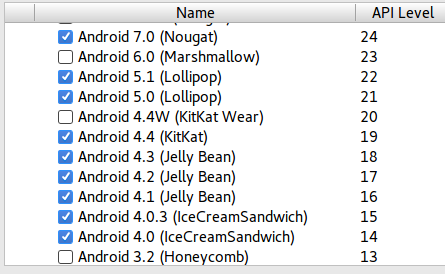
\includegraphics[scale=0.7]{assets/chpt_impl/sdks.PNG}
	\end{center}
\end{figure}

\subsection{Modifying and compiling rosandroid}
\label{impl:compiling_rosandroid}

Since the application developed in this thesis shall work on Android from versions beginning at 4.0.3 we have to modify the rosandroid code on one little detail to make everything work fine. In the created catkin workspace, go to the \textit{src} folder and clone the rosjava and rosandroid repositories there:
\begin{lstlisting}[caption={Cloning the rosandroid and rosjava repositories}]
git clone https://github.com/rosjava/rosjava_core.git
git clone https://github.com/rosjava/android_core.git
git clone https://github.com/rosjava/rosjava_messages.git
\end{lstlisting}

Then line 38 in the file
\begin{lstlisting}[numbers=none]
android_core/android_10/src/org/ros/android/RosActivity.java
\end{lstlisting}

has to be replaced by

\begin{lstlisting}[caption={Change to make to RosActivity.java},firstnumber=38]
public abstract class RosActivity extends android.support.v7.app.AppCompatActivity {
\end{lstlisting}

This gives us the ability to use the already-built features in rosandroid like the automatically displayed activity to connect to a ROS master and built-in node handling even in older Android versions. When changes are made, issue a \textit{catkin\_make} command in the catkin workspace's root directory. \textit{Rosjava} and \textit{rosandroid} will then be built from source and deployed to a \textit{Maven}\footnote{Maven is a dependency and package management system for Java libraries.} repository from where the binaries will be loaded by Android Studio on compile time.

\subsection{Starting the environment}

To start up the development environment with the ROS master, the BioIK service and the \textit{rviz!} simulation of the robot, first the \textit{tams\_cml}\footnote{\url{https://gogs.crossmodal-learning.org/norman.hendrich/tams_cml}} and \textit{bio\_ik\_service}\footnote{\url{https://gogs.crossmodal-learning.org/philipp.ruppel/bio_ik_service}} packages has to be cloned into the catkin workspace, as well as the \textit{tams\_multitouch} package, which has to be copied into the workspace. After \textit{catkin\_make} was executed successfully, the programs are ready to be started. The following commands have to be entered in this order, but within different terminal windows:
\begin{lstlisting}[caption={Commands to start up the development environment}]
roscore
roslaunch tams_multitouch demo.launch
roslaunch tams_f329 4_moveit.launch
rosrun bio_ik_service bio_ik_service
\end{lstlisting}

If interaction with the robot hardware is wanted, the corresponding programs and nodes have to be started according to the file \textit{tam\_cms/tams\_f329/README.txt} within the catkin workspace.

\section{User Interface}
\label{sec:impl:ui}

The user interface of the application was developed according to the considerations made in chapter \ref{chap:concepts}. Additionally it turned out during development, that a basic tele-operation screen for the robot arm would be useful, that enables the user to bring the arm into a defined home position as well as doing simple step-wise manipulation to the robotic arm by moving the desired position of the hand palm by single small steps per button-press. The screen's layout and functionality is described in Section \ref{sec:impl:armteleop}.

The safety interlock button on all screens is immplemented using a \textit{FloatingActionButton}, a predefined conttrol by Android which is designed to float in one corner of the screen above the rest of the screen's contents. To have the \textit{FloatingActionButton} work in the expected way, all screen contents have to be embedded into a \textit{CoordinatorLayout} container. The icon of the button has a \textit{Play} symbol in idle state, in activated state is shows a \textit{Pause} symbol until the button is released. The code to make the interlock button is described in Listing \ref{lst:impl:interlock}. It has to be inserted into the overridden \textit{onStart()} method in every Fragment of the application, in which the functionality shall exist - i.e. every page with controls for the robot.

\begin{lstlisting}[caption={Code for the interlock button}, label=lst:impl:interlock]
@Override
public void onStart() {
	super.onStart();
	
	final FloatingActionButton lockButton = ((FloatingActionButton)getView().findViewById(R.id.lockButton));

	lockButton.setOnTouchListener(new View.OnTouchListener() {
		boolean locked = true;
		
		@Override
		public boolean onTouch(View view, MotionEvent motionEvent) {
			switch(motionEvent.getAction())
			{
				case MotionEvent.ACTION_DOWN:
                        // Code to unlock robot operations
						lockButton.setBackgroundTintList(ColorStateList.valueOf(getResources().getColor(R.color.posOk)));
						lockButton.setImageResource(android.R.drawable.ic_media_pause);
				break;
				
				case MotionEvent.ACTION_UP:
					// Code to lock robot operations
					lockButton.setBackgroundTintList(ColorStateList.valueOf(getResources().getColor(R.color.posNOk)));
					lockButton.setImageResource(android.R.drawable.ic_media_play);
				break;
			}			
			return true;
		}
	});
	
	// ... more code for onStart()
}
\end{lstlisting}

\subsection{Synergy Pages}

\begin{figure}
	\caption{The synergy control screen\label{fig:ui:syn}}
	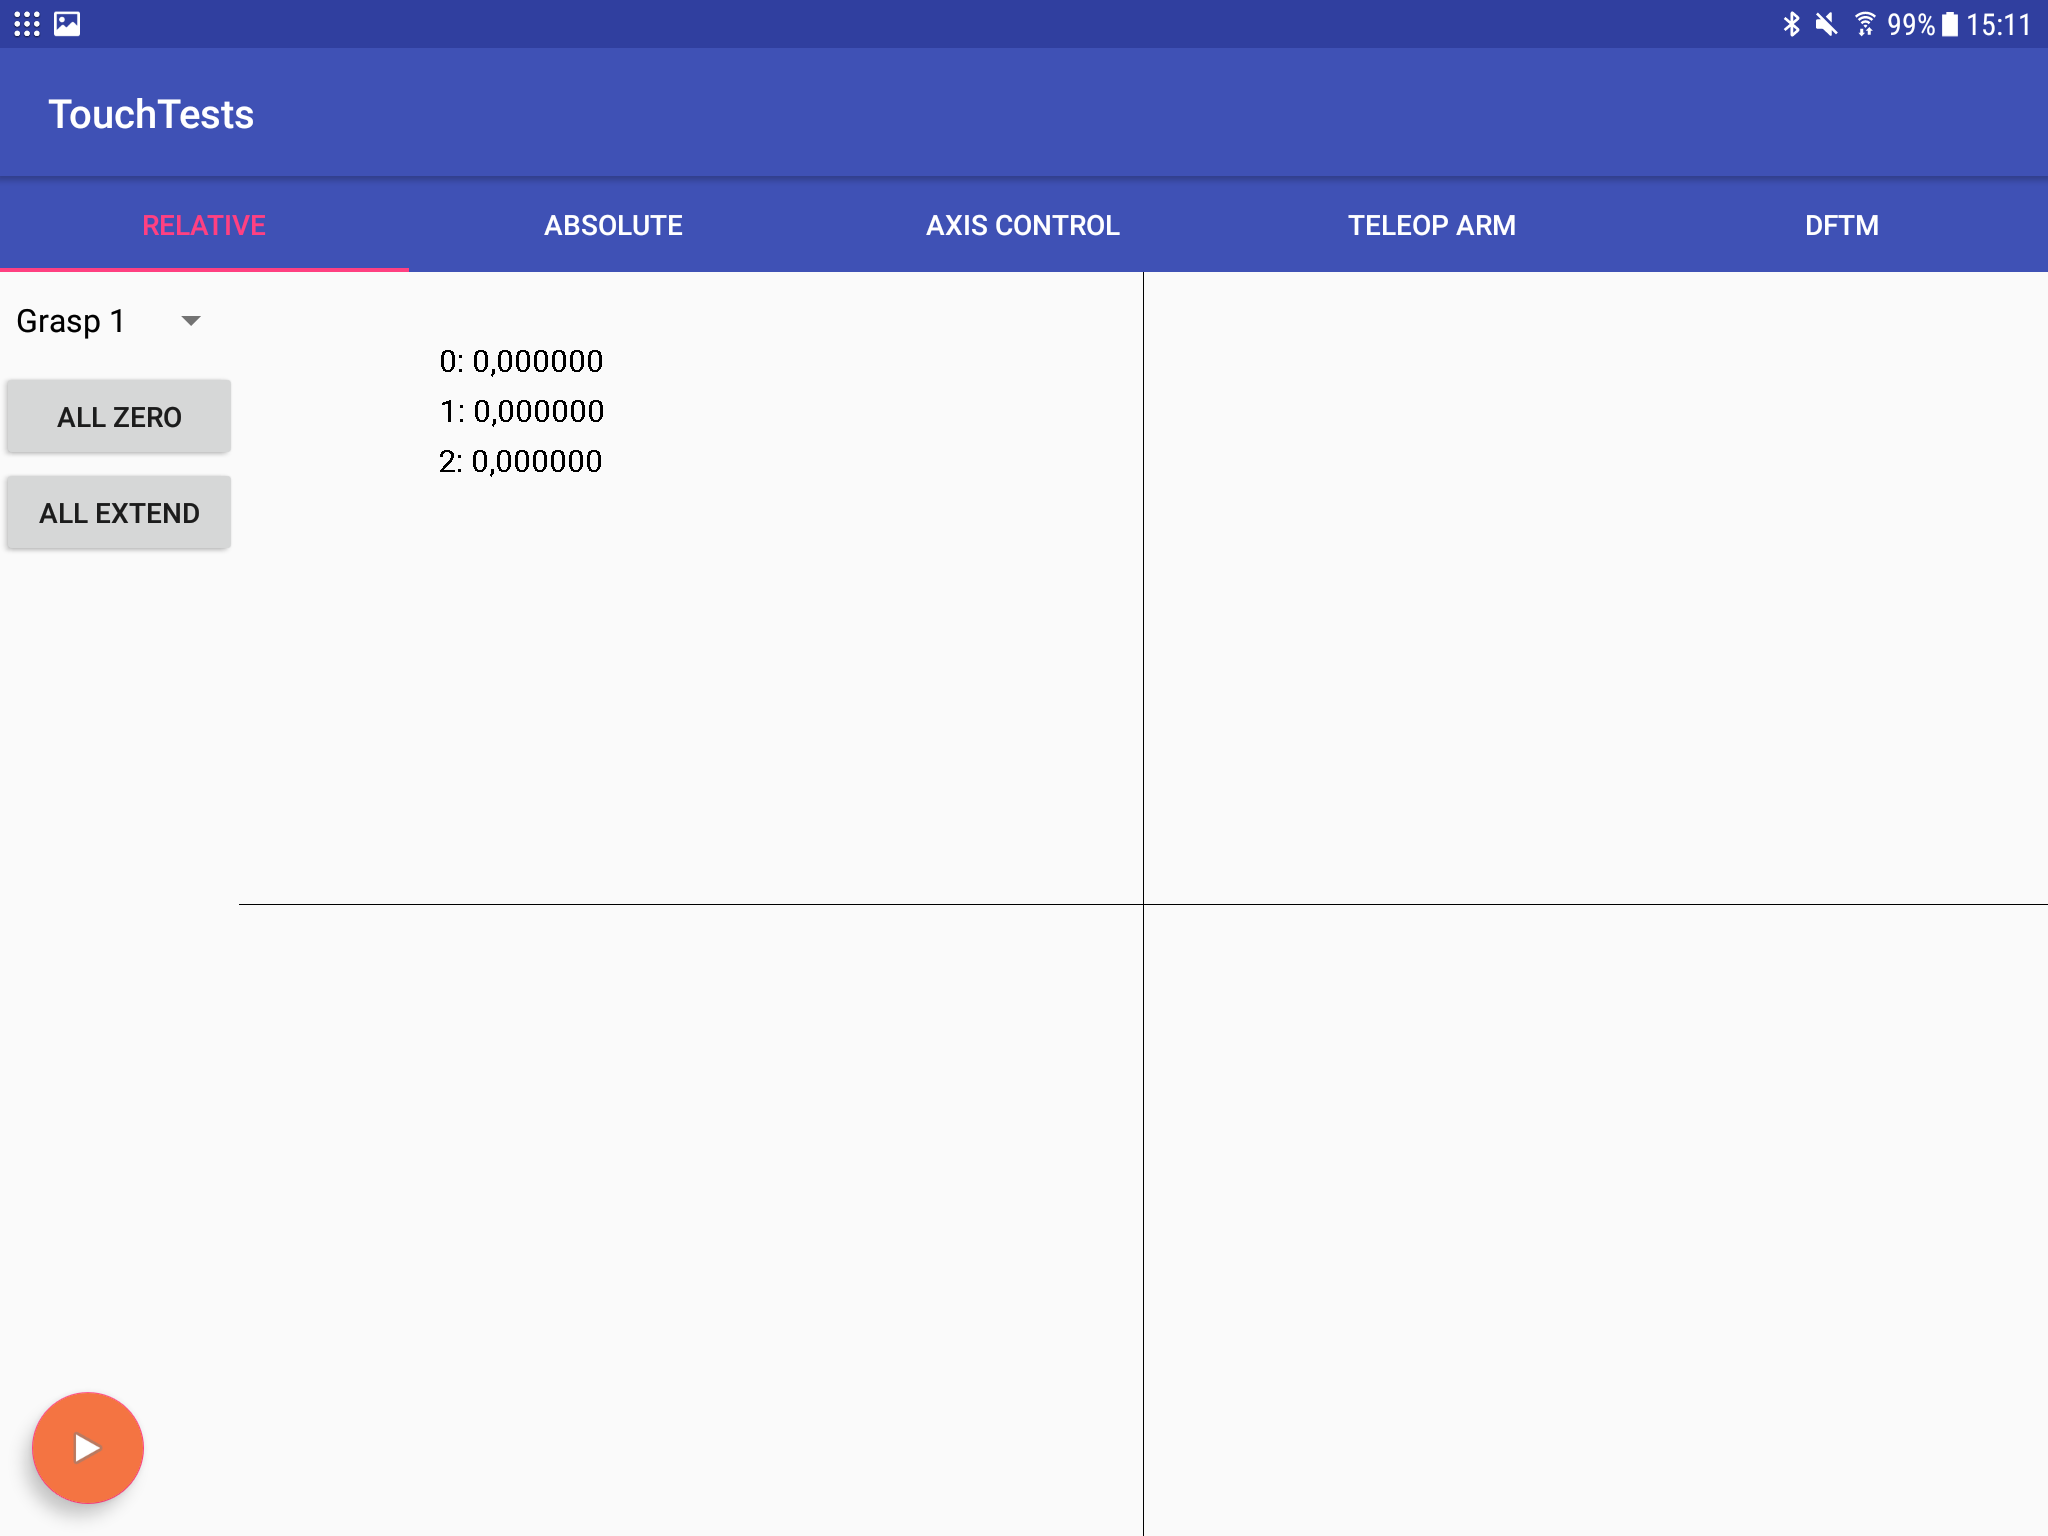
\includegraphics[width=\linewidth]{assets/chpt_impl/syn_blank}
\end{figure}

\begin{figure}
	\caption{display of a two-pointer and a three-pointer gesture on the synergy screen\label{fig:ui:syngest}}
	
	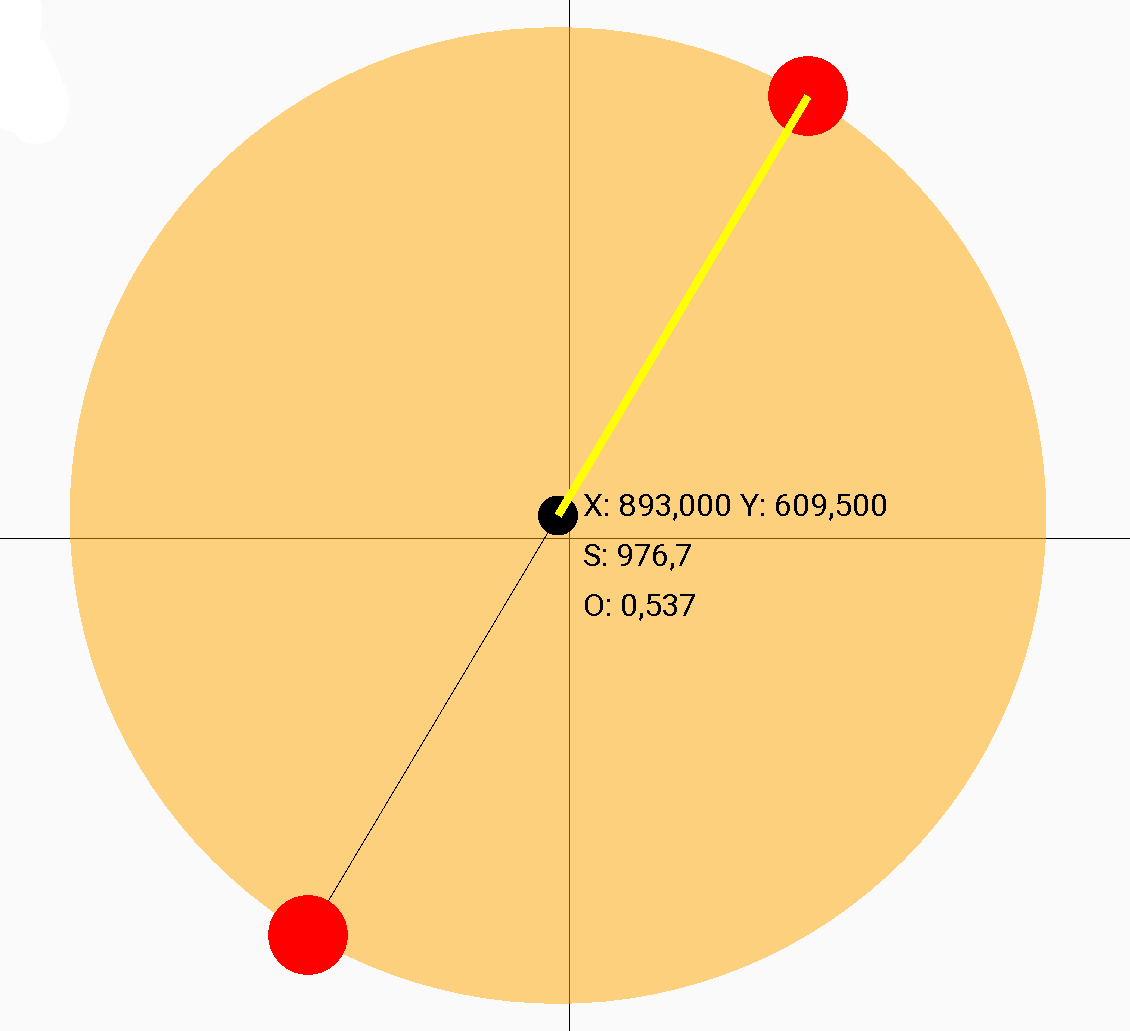
\includegraphics[width=0.5\linewidth]{assets/chpt_impl/syn_2touch}
	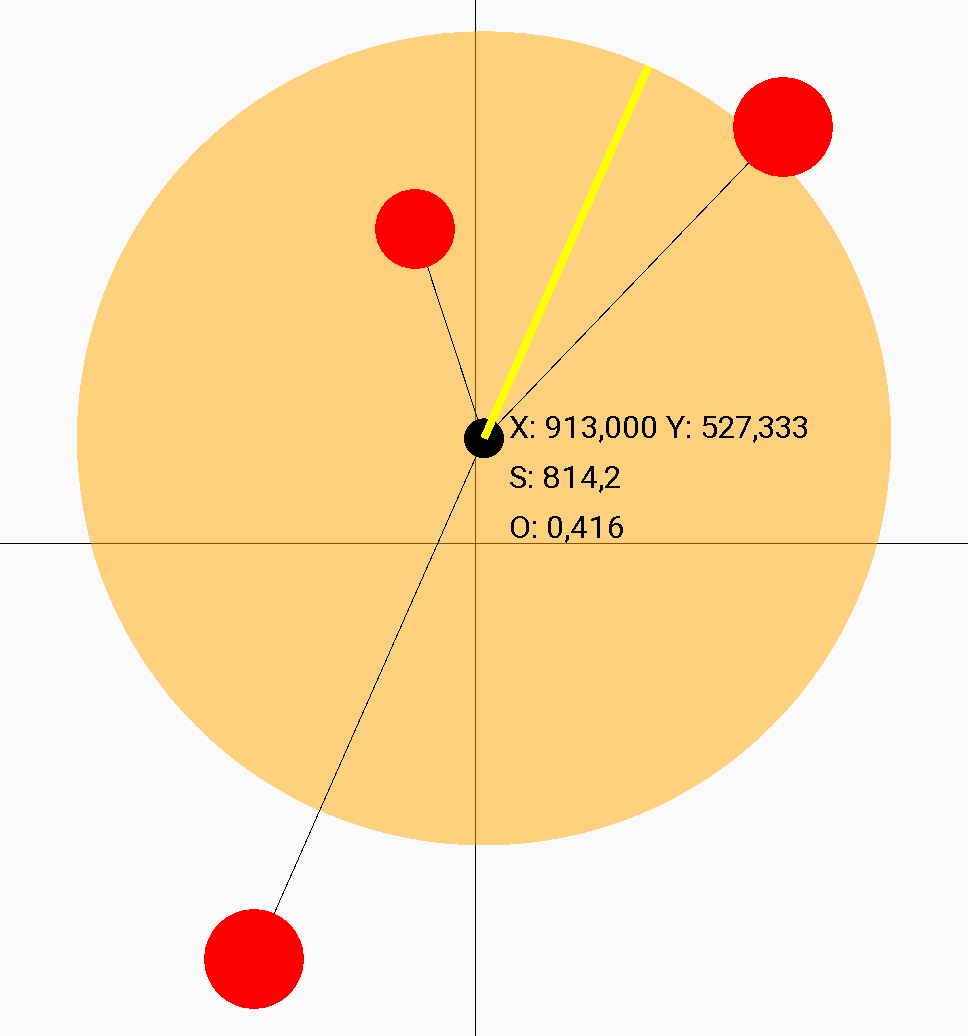
\includegraphics[width=0.5\linewidth]{assets/chpt_impl/syn_3touch}
\end{figure}

The synergy pages are implemented as a mostly blank white page, with a small drop-down control on the left to select the synergy that shall be controlled, as well as a two buttons to set all amplitudes to a known state (i.e. either all zero or all 50). The values of all three controllable amplitudes are displayed in the upper left corner of the control area. The screens for absolute and relative control look the same, which mode is active can be seen in the upper bar with the tab controls. Two lines determine the middle of the control area, which is important for the absolute approach, as the absolute placement of a gesture is important. Figure \ref{fig:ui:syn} gives an impression of how the screen looks on the tablet computer.

Figure \ref{fig:ui:syngest} shows how a two-pointer and a three-pointer gesture is displayed on the synergy pages. While each pointer is marked by a red circle, the center (i.e. the position) of a gesture is displayed as a small black circle, with all pointers being connected to the center by a black line. The orange circle gives an impression of the calculated size of a gesture while the yellow line within the orange circle points in the direction of the orientation which was calculated for a gesture. The calculated values are also displayed in clear text next to the center of a gesture. This is done mainly for debugging purpose, but may also give an interesting insight into the state of a gesture, for example for training purposes. Note that the orientation is not given in degrees, but in radians.

\subsection{Direct Fingertip Mapping Page}

Figure \ref{fig:ui:dfmt} gives an overview of how the DFTM page looks like. It has even less contents than the synergy pages, as no selection has to be made for the current implementation of the DFTM approach. In later iterations it would be sensible to add controls to move the base of the currently workspace on which the fingertips are mapped. As this is not implemented within this thesis, no such controls are displayed. In the same figure an example of how touch pointers are displayed is given for three points. Next to each pointer the name of the link controlled by this pointer is displayed, as well as the coordinates in screen coordinates (i.e. pixels) and world coordinates (i.e. centimeters), both originating in the top-left corner of the white control area. As described more detailed in Section \ref{sec:impl:dfmt}, the pointers are assigned to the links they control in the order in which they are placed on the screen.
If a finger is lifted from the screen (i.e. the touch pointer is de-registered by the Android operating system), one of the following two actions will be performed:
\begin{itemize}
	\item If a pointer of a finger laid down on the screen later than the pointer removed is still present, the pointer is marked as \textit{not present}. Its position does not change, but is still included in IK requests. 
	\item If no such pointer exists, i.e. the lifted pointer was the last present pointer if order of occurrence, it is removed and all pointers laid down after the current one but marked as \textit{not present} are also removed and not included in IK requests anymore.
\end{itemize}

A pointer which is marked as \textit{not present} is displayed as an unfilled circle with a black border (refer to Figure \ref{fig:ui:dfmt_lift} for an example). Once the user places a finger within the black circle, it is registered as this pointer again and the pointer is marked as \textit{present}.

\begin{figure}
	\caption{\label{fig:ui:dfmt}The DFTM screen with three pointers}
	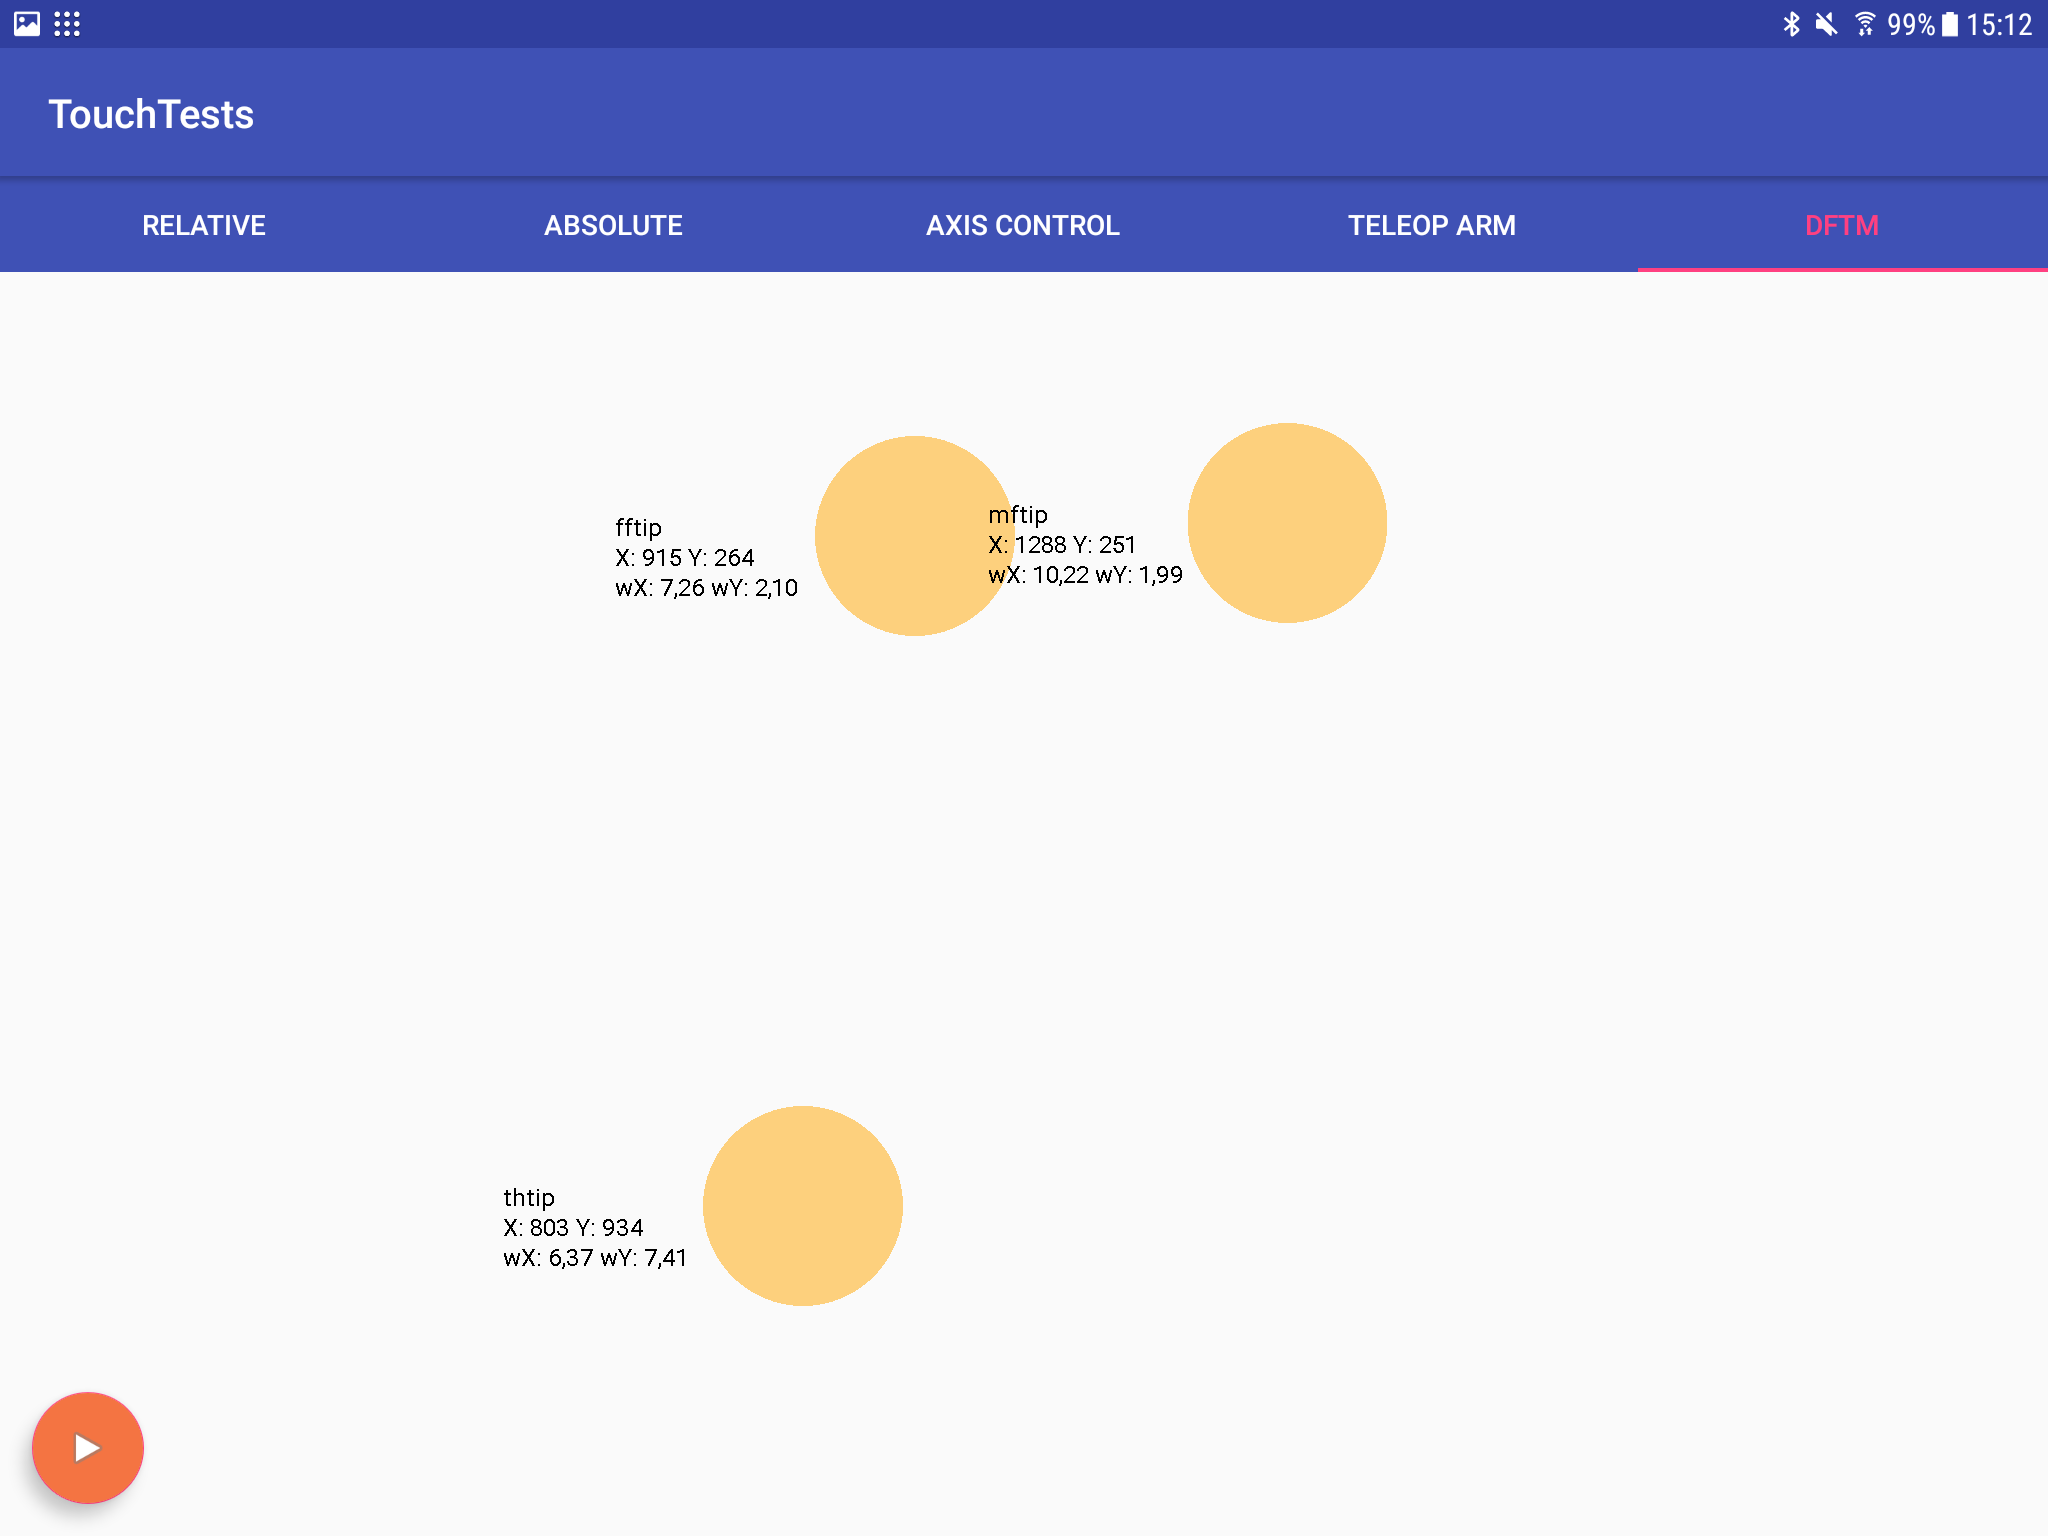
\includegraphics[width=0.9\linewidth]{assets/chpt_impl/dftm}
\end{figure}

\begin{figure}
	\caption{\label{fig:ui:dfmt_lift}The DFTM screen with three pointers, of which one is currently not laid on the screen}
	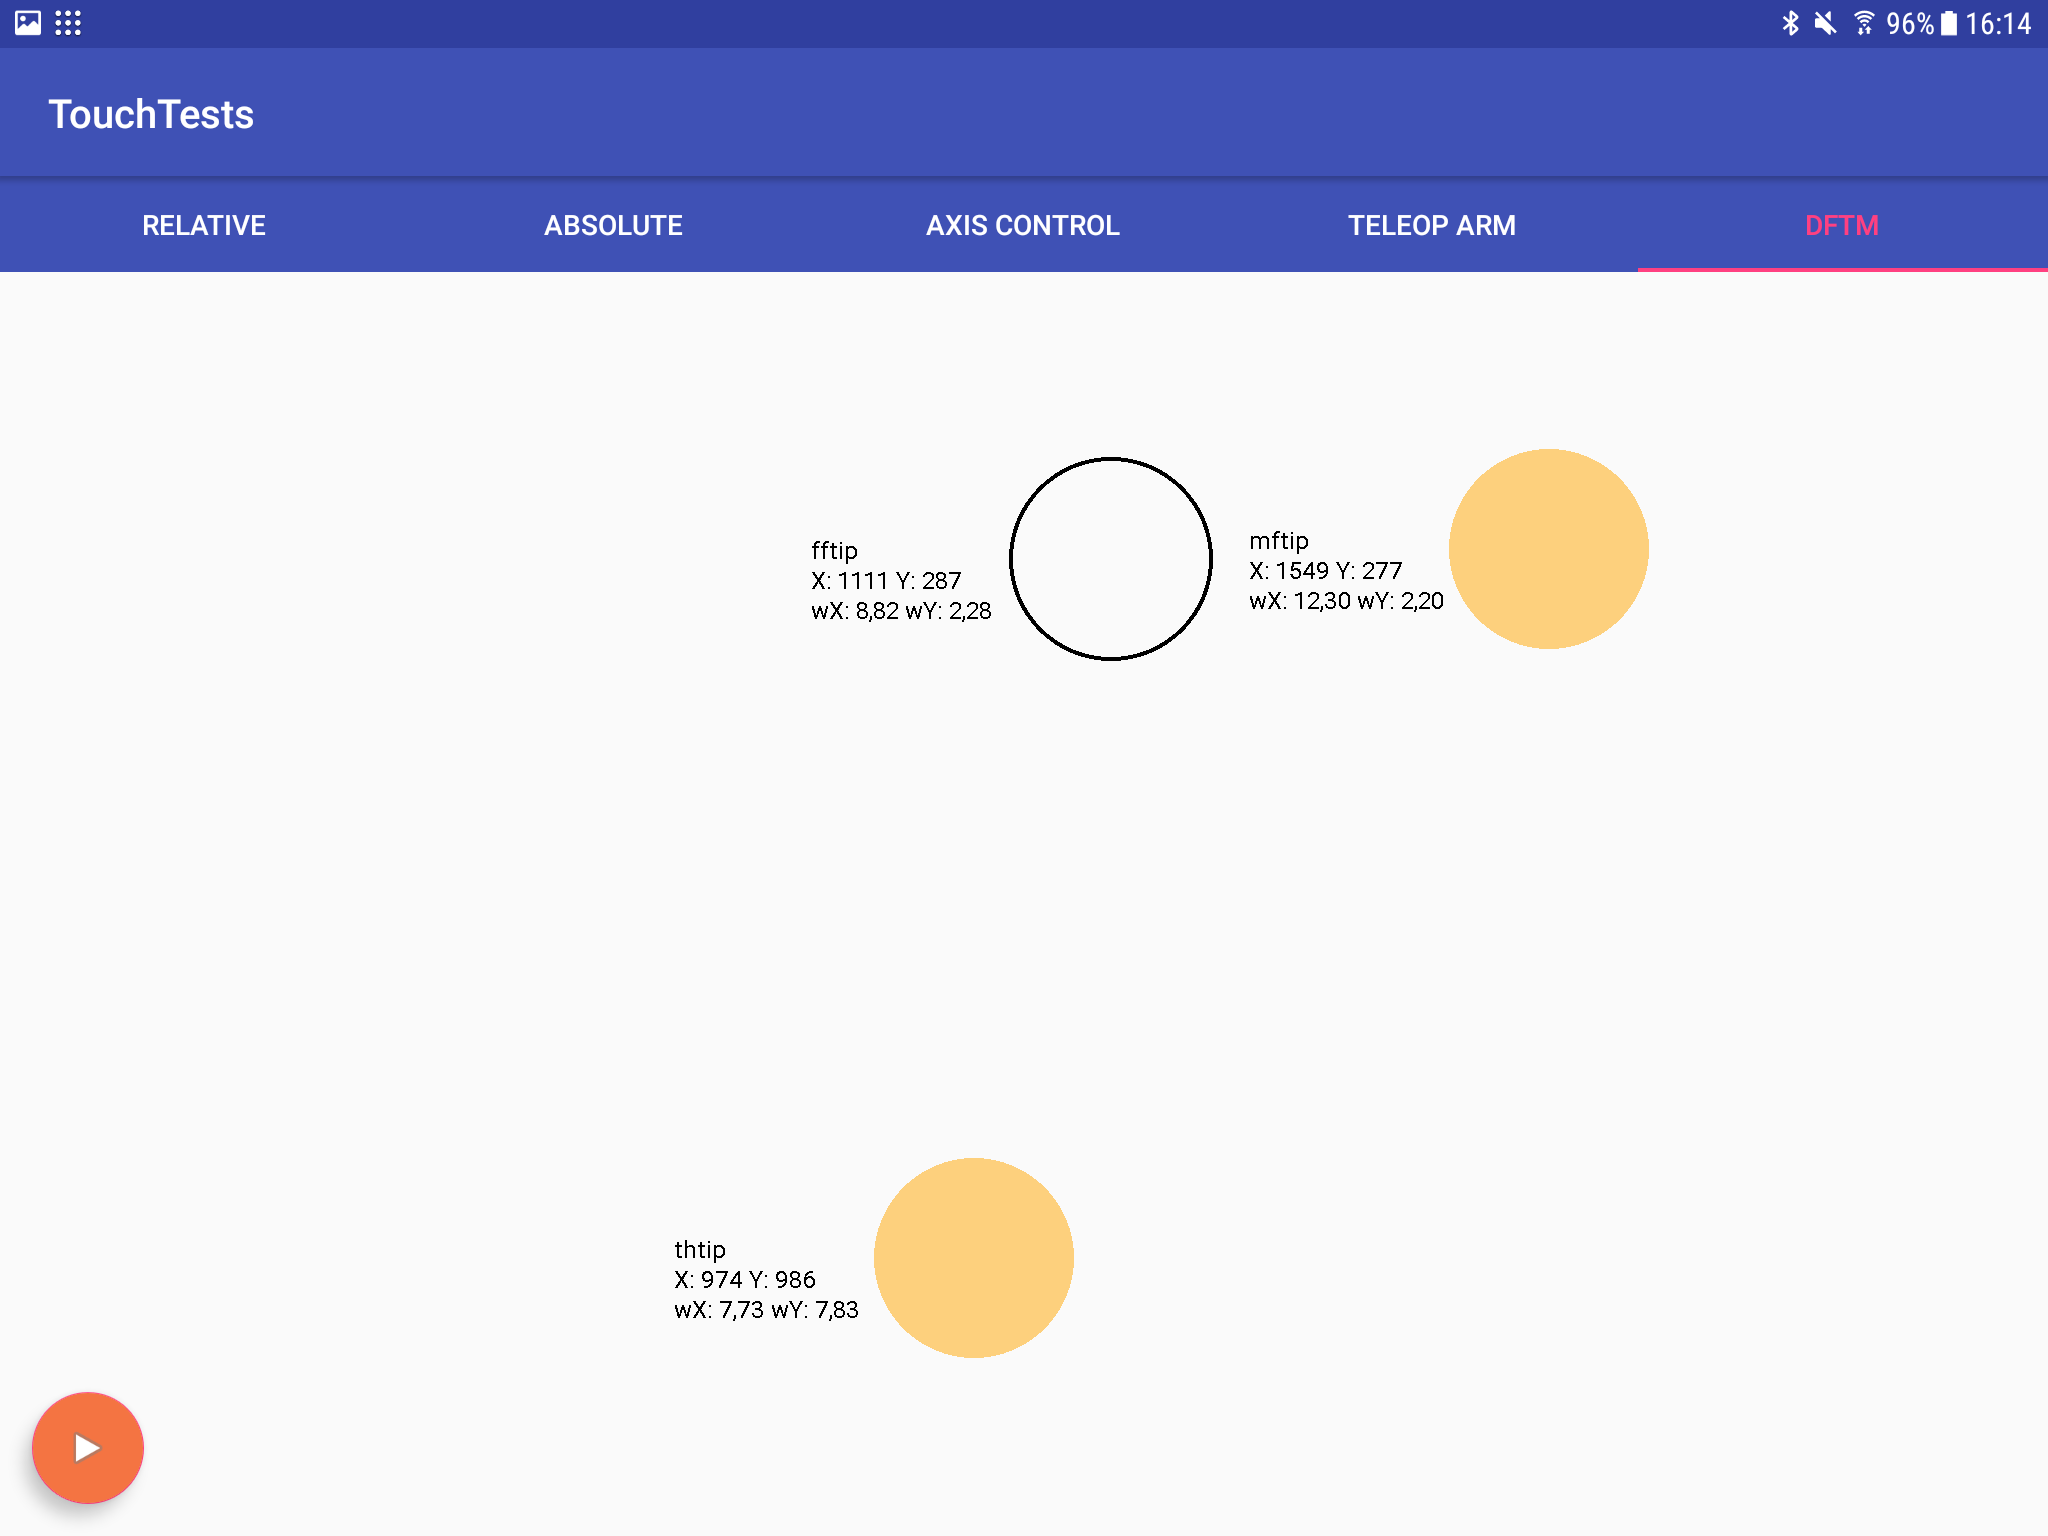
\includegraphics[width=0.9\linewidth]{assets/chpt_impl/dftm_lifted}
\end{figure}

\subsection{Axis Control Page}

The axis control page consists of many \textit{single axis controls} (one for each axis or joint available in the robot, see Figure \ref{fig:ui:axiscontrol}), which -- as defined earlier -- possess two buttons, one to increase and one to decrease the position of the axis or joint. Between those two buttons the target value is displayed (on the top in bold), as well as the currently measured value as received from the robot (in the bottom). The colour between the buttons indicates the magnitude of difference between the target value and the currently measured value as described in Section \ref{sec:conc:axiscontrol}. Axis control widgets for axes that are not controllable (i.e. the first one for every finger except the thumb) have their buttons greyed out and are thus only there to display the current value of the axis.

Two extra buttons are placed on the screen, one labelled \textit{Stop} and one \textit{All Zero}. These buttons are mapped to functionality explained in Section \ref{sec:impl:axism:stop}. The former sets all target values to zero, while the latter copies all currently measured values into the target value, causing the robot to stop all movements.

\begin{figure}
	\caption{\label{fig:ui:axiscontrol}The axis control page}
	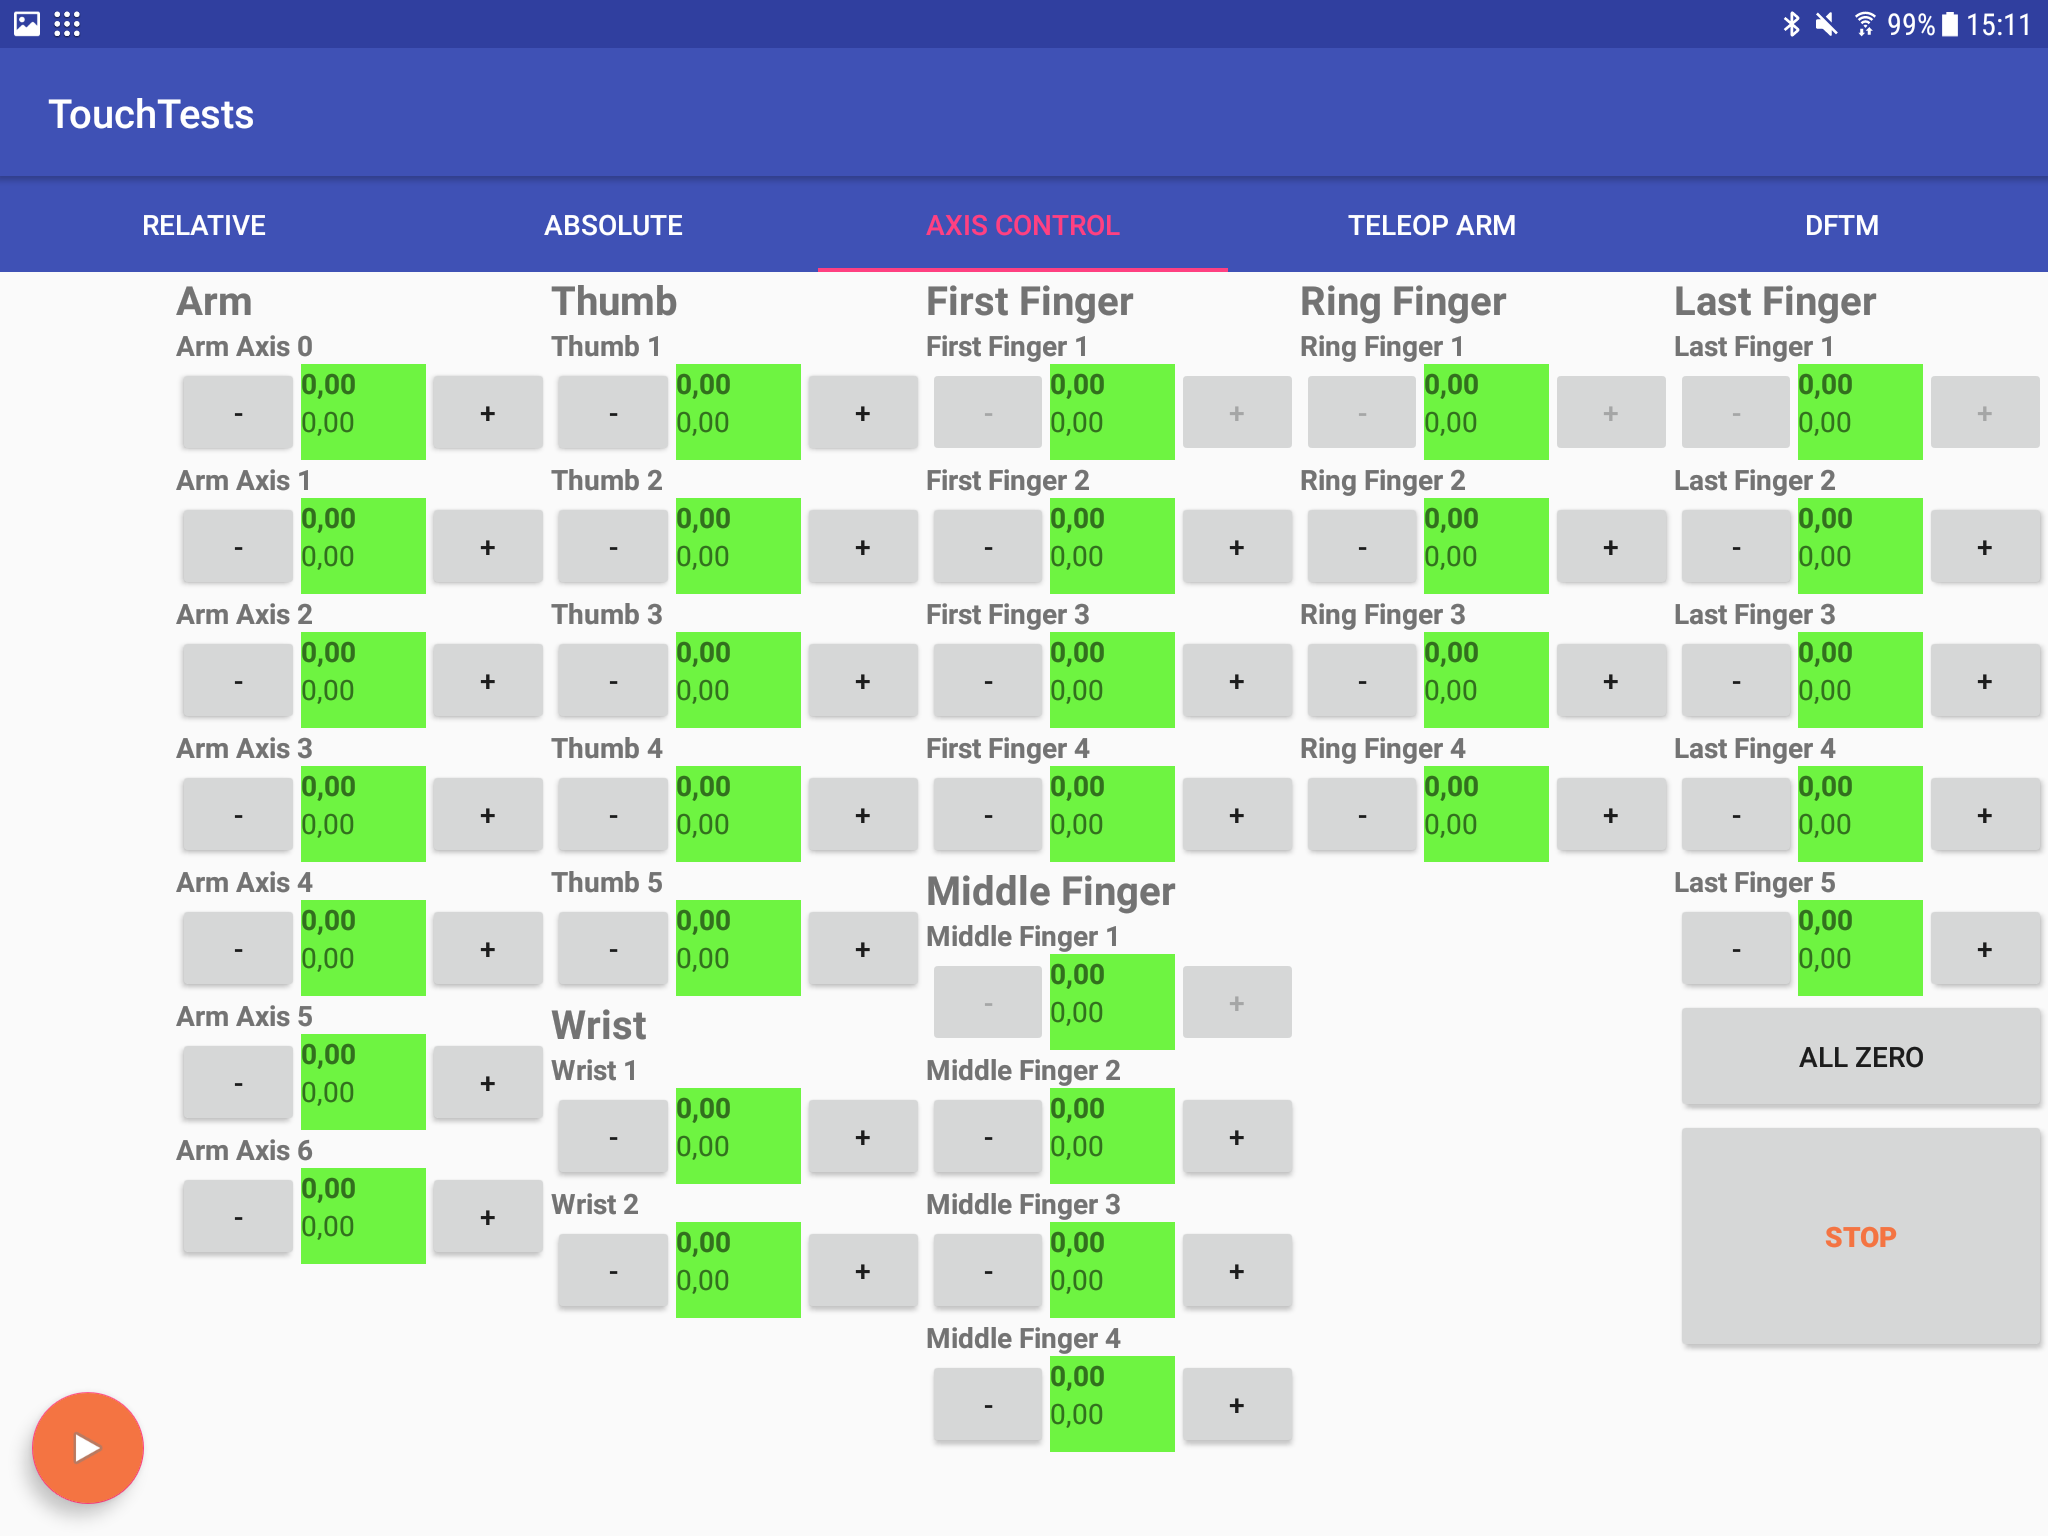
\includegraphics[width=0.9\linewidth]{assets/chpt_impl/axis_control}
\end{figure}

\subsection{Arm Tele-Operation Page}
\label{sec:impl:armteleop}

\begin{figure}
	\caption{\label{fig:ui:teleop}The arm tele-op page}
	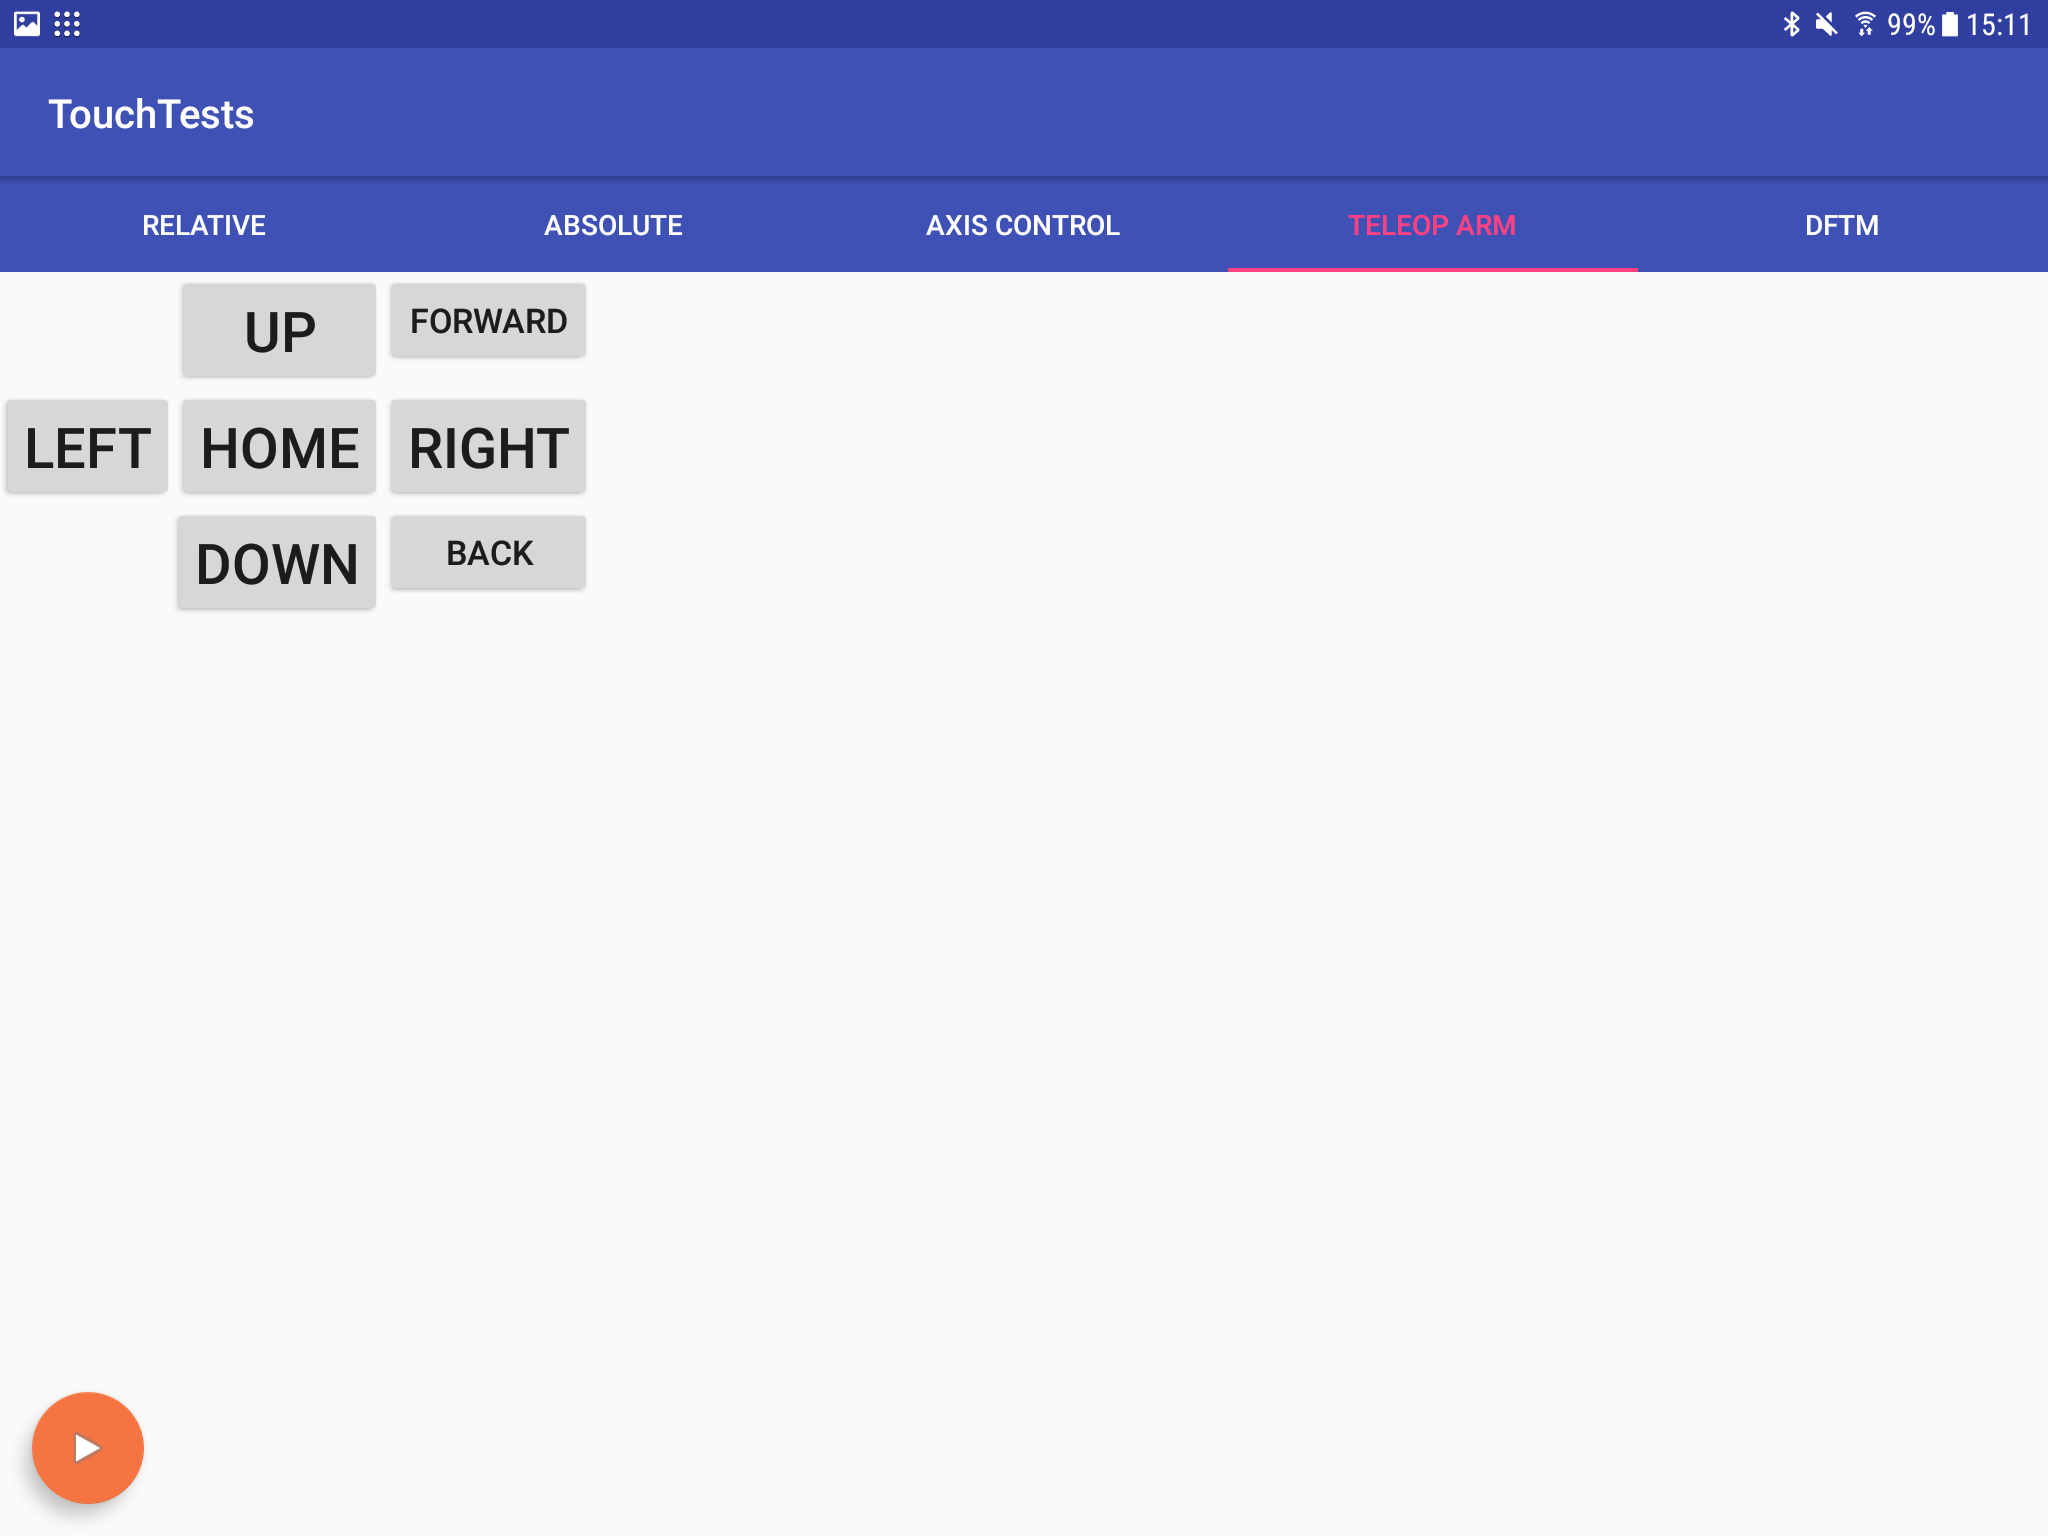
\includegraphics[width=0.9\linewidth]{assets/chpt_impl/teleop}
\end{figure}

As a last page, the arm tele-op page servers as a remote control to move the arm in Cartesian space. The functionality of the \textit{CartesianArmManager} described in Section \ref{sec:impl:armcontrol}. It is important to note that the wording \textit{left, right, forward, backward} are relative to the operators point of view, as standing in front of the robot. Each button press moves the robot's palm by one centimeter into the desired direction. A press on the \textit{Home} button brings the robot into a home position, which is located directly in front of the robot at the border of the table approximately 20cm above the table's plate. This page was implemented for testing reasons, but comes in handy when using the synergy approaches, as the arm should be moved into the \textit{Home} position first before using the gesture control. Doing this using this page is easier than moving every joint on its own using the axis control page. Figure \ref{fig:ui:teleop} gives an impression of the page.

\section{ROS integration}

Thanks to \textit{rosandroid} it is easy to integrate ROS into an Android application. When the libraries are included in the project the main thing to change is that the main activity has to inherit from \textit{RosActivity} instead of the plain Android \textit{Activity} class.

\begin{lstlisting}[caption={Changes to MainActivity}, escapechar=&]
public class MainActivity &\textbf{extends RosActivity}& {
	//...
}
\end{lstlisting}

\begin{wrapfigure}[14]{R}{0.60\linewidth}
\caption{\label{fig:impl:masterchooser}The rosandroid master chooser activity}
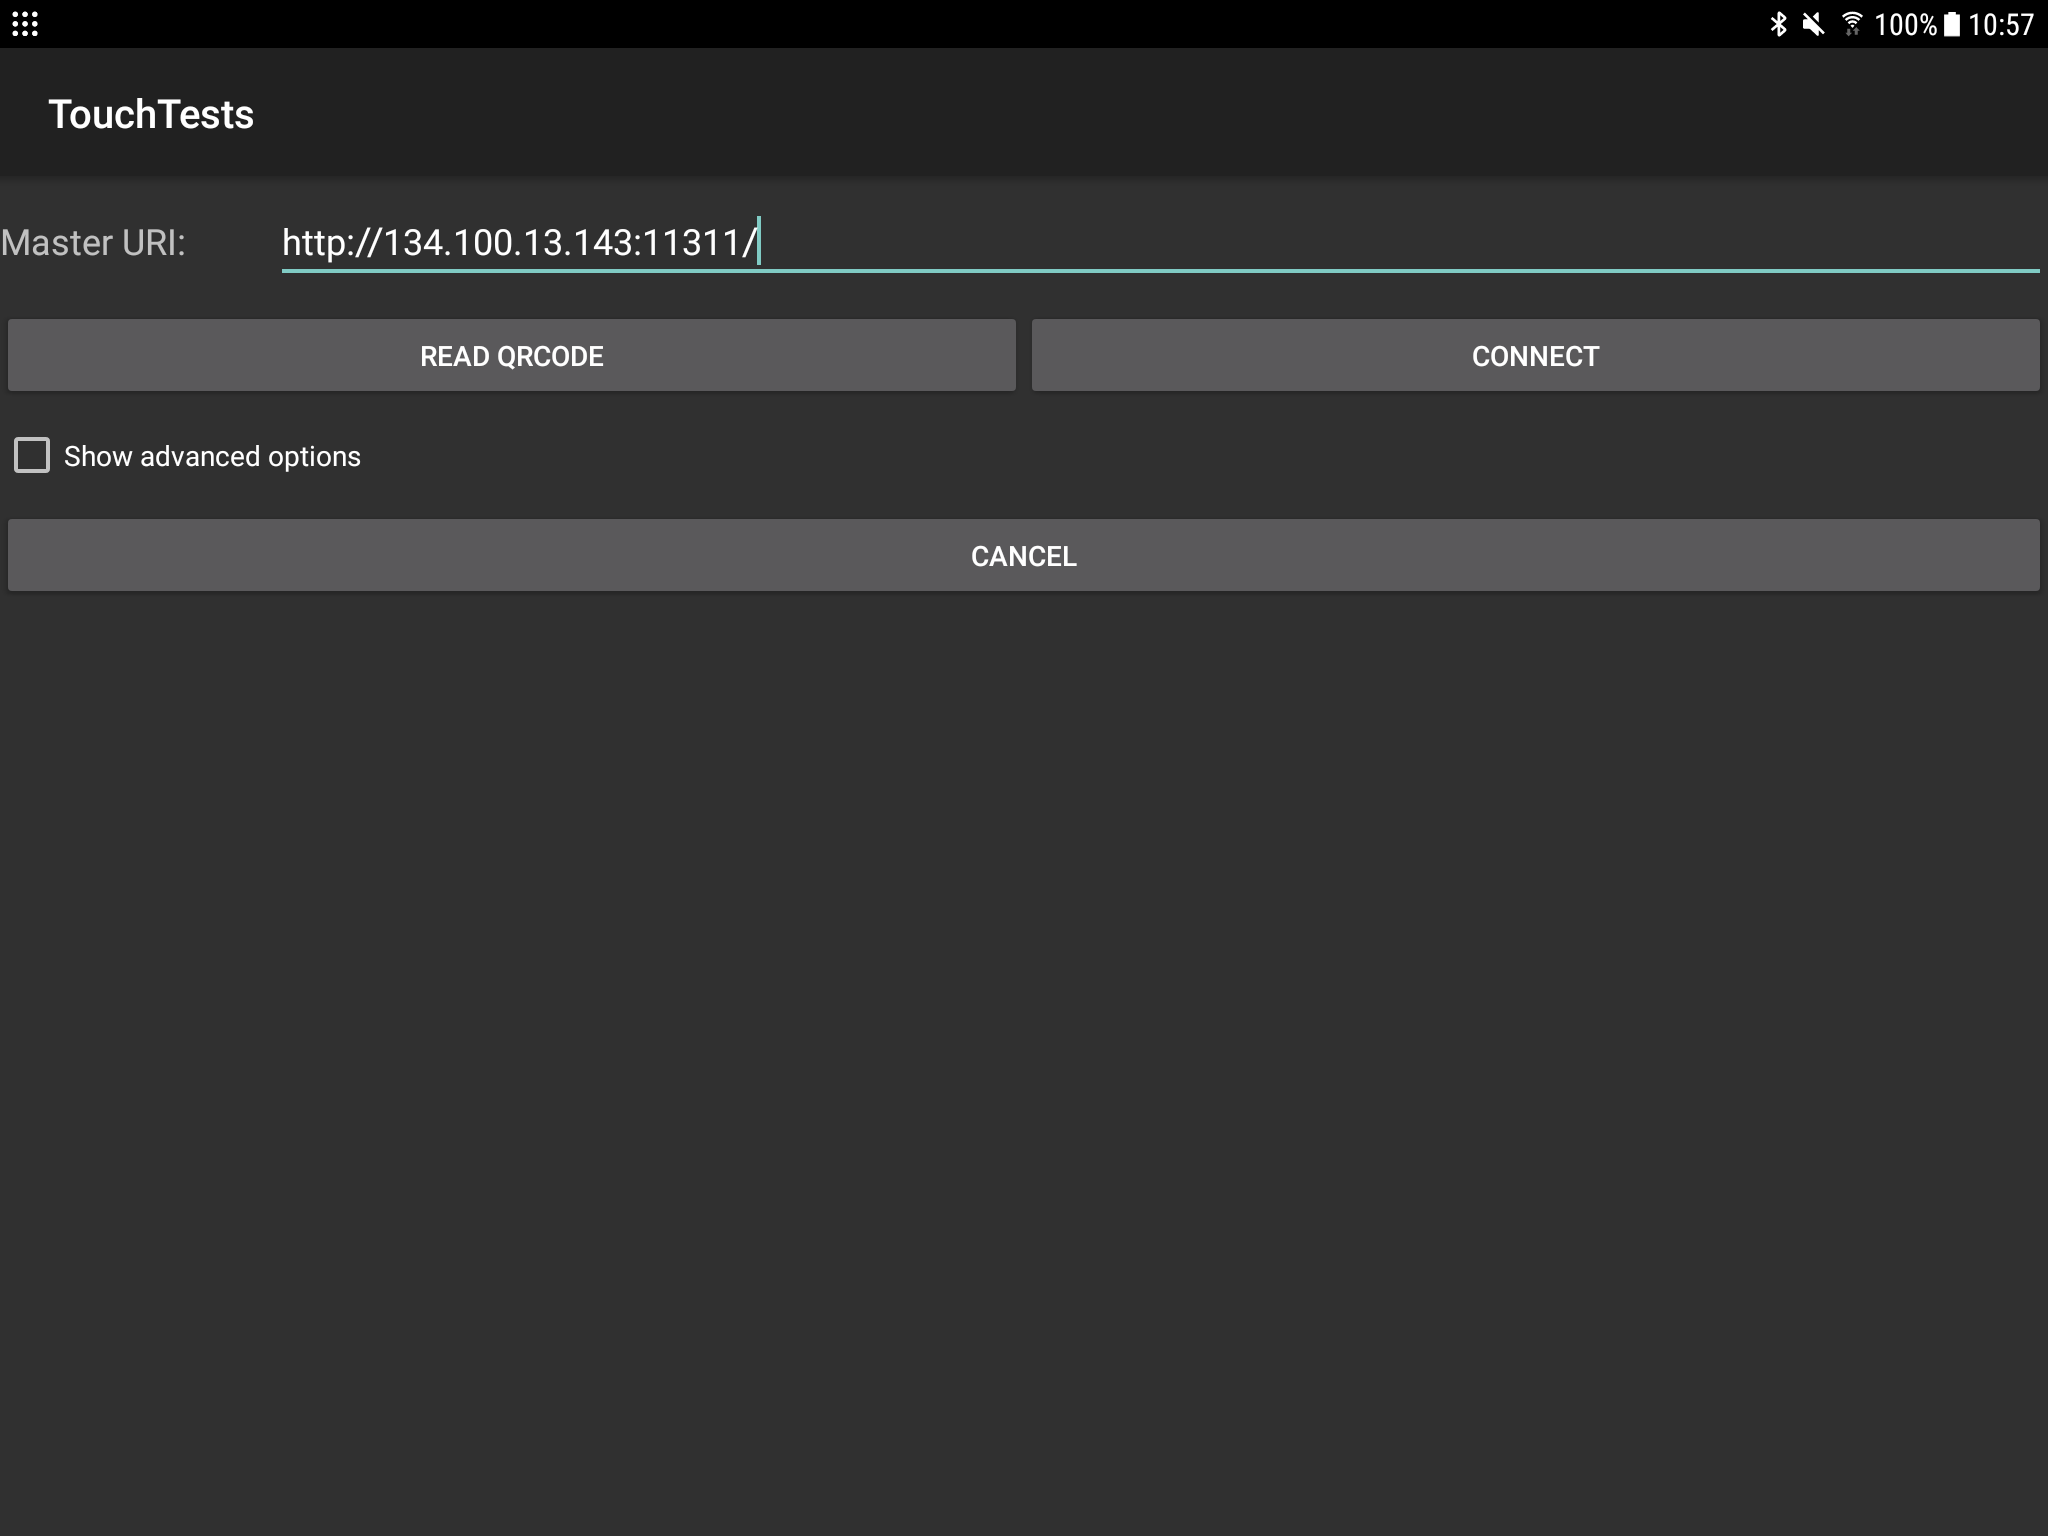
\includegraphics[width=\linewidth]{assets/chpt_impl/masterchooser}	
\end{wrapfigure}

After this change was made, the \textit{RosActivity} implementation takes care about multiple things, beginning with showing a \textit{master chooser}  activity, in which the user can connect to a ROS master node, to handling all connection lifetime events of ROS parts. The \textit{master chooser} activity (see Figure \ref{fig:impl:masterchooser}) lets the user connect to an existing ROS master node. Additionally, it gives the Android application the opportunity to create a dedicated master node on the device itself. As this could affect the overall performance of the application and a lot of functionality has to be run on a more powerful machine, the ROS master is started on a dedicated computer and the Android application connects to this existing master node.

\textit{RosActivity} is an abstract class. To implement it, the \textit{init()} method has to be overriden by inheriting classes. This method is called once the connection to the ROS master node was established and custom nodes can be initialized and connected. All other initialization steps regarding the implemented ROS nodes should also be done here. As shown in Listing \ref{lst:impl:rosconn}\footnote{Information on how to initialize ROS applications was taken from an official rosandroid example found at \url{https://github.com/rosjava/android_core/blob/kinetic/android_tutorial_pubsub/src/org/ros/android/android_tutorial_pubsub/MainActivity.java}}, first an instance of the \textit{C5LwrNode} is created and then assigned to all instances that consume functionality of it (\textit{AxisManager}, \textit{CartesianArmManager}, \textit{DfmtProxy}). After all this is done, the node is registered with the ROS master node. Details on the initialization of the \textit{C5LwrNode} node can be found below in this section. In theory, multiple nodes can be started and registered with the master within one application.

\begin{lstlisting}[caption={Initialization of the ROS connection}, label={lst:impl:rosconn}]
@Override
protected void init(NodeMainExecutor nodeMainExecutor) {
	axisManager = AxisManager.getInstance();
	
	node = new C5LwrNode("/joint_states", "/hand/joint_goals", "/lwr/jointPositionGoal");
	node.addJointDataListener(axisManager);
	
	axisManager.setRobotNode(node);
	CartesianArmManager.getInstance().setNode(node);
	DftmProxy.getInstance().setNode(node);

	NodeConfiguration cfg = NodeConfiguration.newPublic(getRosHostname(), getMasterUri());
	nodeMainExecutor.execute(node, cfg);
}
\end{lstlisting}

\subsection{The C5LwrNode class}

The class \textit{C5LwrNode} inherits from \textit{AbstractNodeMain}, which already offers the very basic lifetime functionality of a ROS node. Some methods have to be implemented by the developer, like \textit{getDefaultNodeName()}, which determines the name of the ROS node as it is registered with the ROS master. In the \textit{onStart()} method, all start-up procedures are implemented, like registering topic subscriptions as well as creating publishers and \textit{service clients}. Within the \textit{onShutdown()} method, all resources created before (subscribers, publishers, service clients) shall be closed and deleted to ensure a clean de-registration from the ROS master and a clean shut-down of the application. The start-up code for the ROS node can be seen in Listing \ref{lst:impl:c5lwrnode}.

\begin{lstlisting}[caption={Startup of the C5LwrNode}, label=lst:impl:c5lwrnode]
@Override
public GraphName getDefaultNodeName() {
	return GraphName.of("ba_android/c5lwrnode");
}

@Override
public void onStart(ConnectedNode connectedNode) {
	cNode = connectedNode;
	handJointStatePub = connectedNode.newPublisher(handPublishTopic, JointState._TYPE);
	armJointStatePub = connectedNode.newPublisher(armPublishTopic, RMLPositionInputParameters._TYPE);

	jointStateSubsc = connectedNode.newSubscriber(subscribeTopic, JointState._TYPE);
	jointStateSubsc.addMessageListener(/* ... */);

	try {
		ikService = connectedNode.newServiceClient("/bio_ik/get_bio_ik", bio_ik_msgs.GetIK._TYPE);
	} catch (ServiceNotFoundException e) {
		ikService = null;
		e.printStackTrace();
	}
}
\end{lstlisting}

The methods that are used to offer the functionality of the \textit{C5LwrNode} are denoted in Listing \ref{lst:impl:c5lwrik}. Because arm and hand joints have to be published to different topics, the \textit{handleJointData()} method calls either \textit{publishHand()} oder \textit{publishArm()}, depending on the parameter \textit{jointType} which is passed by the caller indicating the type of the joint data given. The two methods to request IK solutions from the BioIK service are relatively similar, as both initialize the request with the current robot state passed as a parameter and add a \textit{MinimumDisplacementGoal} to hint the IK solver that a solution is desirable where the least possible movement in all axes is done. The number of attempts is set to $1$, the time-out to find a solution is set to $10ms$ for the palm position and $500ms$ for the fingertip positions. The main difference is that, while for the palm only one \textit{PoseGoal} is added, containing the desired pose of the palm constructed by the x, y, z position and \textit{Quaternion} rotation as passed by the caller, in the method to get a solution for multiple fingertips one \textit{PositionGoal} is added for each fingertip as well as an \textit{OrientationGoal} to have the palm of the robotic hand always point in the same direction. In \textit{GetIKJointsFingertips()}, the \textit{fingertips} parameter contains a map with the link names (e.g. \textit{fftip}, \textit{thtip}...) as key values and the desired 3-dimensional position of the link.

\begin{lstlisting}[caption={C5LwrNode interface},label=lst:impl:c5lwrik]
public class C5LwrNode extends org.ros.node.AbstractNodeMain implements RobotJointDataReceiver {
	private void publishHand(HashMap<String, Double> data);
	private void publishArm(HashMap<String, Double> data);
	
	@Override
	public void handleJointData(int jointType, HashMap<String, Double> data);
	
	public void GetIkJointsPalm(Map<String, Double> currentState, 
		String[] lockedAxes, 
		double x, double y, double z, 
		double rotx, double roty, double rotz, double rotw,
		ServiceResponseListener<GetIKResponse> hdl);
	
	public void GetIKJointsFingertips(Map<String, Double> currentState,
		Map<String, PointInSpace> fingertips, 
		ServiceResponseListener<GetIKResponse> hdl);
}

\end{lstlisting}

\section{The AxisManager}

The most important and most central functionality of the overall application is offered by the \textit{AxisManager} class. It is responsible for holding the current joint angles for all joints in memory, as well as the current target values along multiple other bits of information about each axis or joint. Joints are more generically called \textit{axis} within the \textit{AxisManager}, so this wording will be adopted in the rest of this section.

\subsection{AxisInformation}

All information about an axis is stored in a \textit{AxisInformationImpl} object. This class implements the \textit{AxisInformation} interface, which is returned when axis information shall be given to callers in a read-only manner. The \textit{AxisInformation} interface is given in Listing \ref{lst:impl:axisinformation}. All the information stored about an axis is accessible here. In particular, this is: 
\begin{itemize}
	\item the identifier of an axis, i.e. a string literal containing the name at which the axis or joint is known to the ROS nodes.
	\item the maximum speed the axis may move at.
	\item the target value to which the axis shall be currently moved.
	\item the value representing the axis' current position.
	\item the value representing the axis' \textit{current target value} (see Section \ref{sec:impl:axismovements} for details).
	\item the minimum and maximum values the axis may have as position value.
	\item flags indicating whether the axis is enabled and moving.
	\item an integer representing the type of an axis. Allowed types are \textit{JointType.ARM} and \textit{JointType.HAND}.
\end{itemize}

\begin{lstlisting}[caption={The AxisInformation interface}, label=lst:impl:axisinformation]
public interface AxisInformation {
	String getIdentifier();
	
	double getMaxSpeed();
	double getTargetValue();
	
	double getMaxValue();
	double getMinValue();
	double getCurrentTargetValue();
	double getCurrentValue();
	boolean isMoving();
	double getSpeed();
	boolean isEnabled();
	int getJointType();
}
\end{lstlisting}

All the information is held within the \textit{AxisManager}, referenced by the axis identifier. Manipulation of the data is only done through calls to the \textit{AxisManager}, to give it full control about what happens with all axes. The difference between \textit{AxisInformation} and the concrete implementation \textit{AxisInformationImpl} is, that the implementation has a setter function for every property. All calculations are done within the \textit{AxisManager} itself.

\subsection{AxisManager timer tick}

The \textit{AxisManager} is designed to work fully asynchronous. All information about axes' target values is stored in the according \textit{AxisInformation} object, but only processed from within the main timer event used in \textit{AxisManager}. The timer is set to a frequency of $f_{am} = 10Hz$. This value can easily be changed by altering the static constant field \textit{UPDATE\_FREQ} in the \textit{AxisManager} task. An implementation of a timer is used which gives the ability to schedule an event at a fixed rate. \textit{java.util.Timer} is able to ensure the desired frequency is reached in the long run by slightly alternating the delays between two executions\cite{AndroidTimer2018}. This is important to have axis movements and publishing done at the correct speed and frequency. To use with functionality, the method \textit{scheduleAtFixedRate()} on the timer has to be used. 

All calculations regarding axis movements (Section \ref{sec:impl:axismovements}) are done within the timer tick only. After all calculations have been done the current joint angles are all sent to the \textit{C5LwrNode} to be published over ROS (see Section \ref{sec:impl:aximgrros}).

\subsection{Initialization}

When the application starts or is resumed from a sleeping device (i.e. the screen went off), the \textit{AxisManager} is initialized. This means that it blocks all actions until it has received a specific number of joint states from the \textit{C5LwrNode}. This measure was implemented to prevent the application from sending joint data to a non-existent robot and to initialize the joint data within memory with the current state of the robot. After 20 samples (\textit{JointState}s) have been received, the values are copied into the target values for each axis.
Initializing all joint target values with 0 is obviously not a good choice, as the robot would then go to this position out of any state it is currently in, causing unwanted movements and behaviour. During initialization a modal dialog is shown, blocking all user interaction with the graphical user interface.

\subsection{Axis movements}
\label{sec:impl:axismovements}

The main task of the \textit{AxisManager} is managing movement of all axes in a safe manner. To accomplish this, it restricts the movement for each axis to the maximum speed stored within the \textit{AxisInformation}. Two main modes are available for movement. The first one is by enabling a constant movement of an axis at a specified speed. The second is by setting target values, which the axis will then be moved to at a maximum speed defined on a per-axis basis in the \textit{AxisInformation} object.

\subsubsection{Constant movement}

To set an axis to constant movement at a constant speed, the method
\begin{lstlisting}
public boolean startMoving(String identifier, double speed);
\end{lstlisting}
on \textit{AxisManager} can be called. The parameter \textit{identifier} is filled with the string literal identifying an axis, while \textit{speed} indicates the speed at which the axis shall move. Since only rotational joints are present it the used set-up, the speed (as well as the maximum speed defined in \textit{AxisInformation}) is denoted in $\frac{\text{degrees}}{s}$. The movement speed can be given either positive or negative, depending on the direction the axis shall move in. With this function call, only the information that the axis shall move is stored in \textit{AxisInformation}, actual movement takes place in the timer event, in which the movement speed in clipped to the maximum speed defined for an axis and then divided by the frequency of the timer tick $f_{am}$. In each timer tick event, the position of an axis moving at speed $v$ is altered by $\frac{v}{f_{am}}$. When a constantly moving axis reaches its limit value, the \textit{moving}-flag is not reset, but as the position for an axis is clipped to its maximum and minimum values, no actual movement is done any further. To cancel a constant movement of an axis, simply
\begin{lstlisting}
public boolean stopMoving(String identifier);
\end{lstlisting}
has to be called with the string literal identifying the axis which shall be stopped.

\subsubsection{Setting target values}

The most common use-case in the application is that different parts of the program set values for each axis to be reached. Instead of simply sending the values received by other parts of the program to the robot over ROS, the axis manager implements a safety feature limiting the movement speeds of an axis at a maximum speed. To accomplish this another variable is introduced in \textit{AxisInformation}, the \textit{current target value}. While the \textit{target value} of an axis determines the desired position where the axis shall be at the end, the \textit{current target value} is the value which is actually sent to the robot. The \textit{current target value} is modified in the timer tick.

To change the target value of an axis, \textit{setTargetValue()} has to be called. The signature of the method is
\begin{lstlisting}[caption={Signature of setTargetValue()}, label=lst:impl:settargetval]
public boolean setTargetValue(
	String identifier, 
	double value, 
	boolean force,
	boolean notifyObservers
);
\end{lstlisting}
A call to this method sets the target value $p_t$ of the axis identified by \textit{identifier} to \textit{value}. If \textit{force} is \textit{true}, the smooth movement mechanism described below is overridden and the current target value $p_c$ is directly set to $p_t$ as well. Setting \textit{notifyObservers} to \textit{true} results in the observers of \textit{AxisManager} being notified about the new target value. As the notification often has UI updates as a consequence, it is sensible to notify observers on setting the last value only, not on changing of every value. For convenience, multiple overloads of this method exist, setting either \textit{notifyObservers} to a default of \textit{true}, or \textit{notifyObservers} to \textit{true} and \textit{force} to \textit{false}.

With $p_t$ being the target value as set in \textit{AxisInformation}, $p_c$ the current target value, $v_{max}$ the maximum speed of an axis and $f_{am}$ the frequency of the main timer tick in \textit{AxisManager}, the procedure to move an axis within the main timer tick is as follows:

First, $\Delta p$ is calculated, which is the maximum value change within one timer event, thus
\begin{equation*}
\Delta p = \frac{v_{max}}{f_{am}} \, .
\end{equation*}
Second, the \textit{current target value} is updated as follows:
\begin{equation*}
p_{c,new} = \left\{ 
\begin{array}{ll}
p_t & |p_t - p_c| < \Delta p \\
p_c + \Delta p & |p_t - p_c| > \Delta p \land p_t > p_c \\
p_c - \Delta p & |p_t - p_c| > \Delta p \land p_t < p_c
\end{array}
 \right.
\end{equation*}

The calculated value $p_{c,new}$ is then stored into the \textit{AxisInformation} for each axis.

\subsection{Passing axis data to ROS}
\label{sec:impl:aximgrros}

After each execution of the movement processes described in Section \ref{sec:impl:axismovements}, the newly calculated values are published to the ROS nodes controlling the robot arm and hand. As angles for arm joints and hand joints have to be published to different ROS topics, two calls have to be made. The interface \textit{RobotJointDataReceiver}, which is implemented by \textit{C5LwrNode} has a method
\begin{lstlisting}
void handleJointData(int type, HashMap<String, Double> data);
\end{lstlisting}
accepting the joint type as the first parameter. The ROS node implementation will choose the topic to publish the data to by the given type identifier.

At the end of the timer event in \textit{AxisManager}, first all \textit{current target values} for arm joints are taken from the list of \textit{AxisInformation}. The angle values are converted to radians and put into a Map, which has the axis identifier as the key and the angle of the corresponding axis as value. \textit{handleJointData()} is then called with \textit{JointType.ARM} and the created map. The same procedure is then executed for all \textit{AxisInformation}s with the type \textit{JointType.HAND}.

\subsection{Stopping movement and setting all axes to zero}
\label{sec:impl:axism:stop}
Two extra functions are implemented in \textit{AxisManager}. The first,
\begin{lstlisting}
public void copyCurrentValuesToTarget();
\end{lstlisting}
takes all values currently stored as \textit{current value} in \textit{AxisInformation} and copies them into the \textit{target value} and \textit{current target value} fields. This mainly takes the current robot state and copies it into the target state, causing all movements to stop. This is especially useful when the robot cannot reach a position defined by the target position. This is for example the case when all joints of the hand shall be set to $0^\circ$, as some joints are not able to completely reach this value. Copying the currently measured value into the target value stops the robot from trying to reach the actual desired value and, by this, prevents the hardware from being damaged by trying to reach a non-reachable position for too long.

The second special method is
\begin{lstlisting}
public boolean setAllZero(boolean force);
\end{lstlisting}
which sets all axis \textit{target values} to 0. If \textit{force} is \textit{true}, the \textit{current target value} is also set to 0. \textbf{Extreme caution has to be used when calling this function!} The robot will move all joints to a position of 0 degrees either immediately (\textit{force} is \textit{true}) or smoothly. The shortest way in joint space from the current state of the robot to $\vec{0}$ may cause damage to the robot or its environment. This function was implemented to bring the robot to a known state using the axis control page. If the corresponding button is pressed, it is called only after the user has stated that he is aware of the possible dangers.

\subsection{Enabling and Disabling}

The \textit{AxisManager} can be enabled or disabled. In the disabled state, all calls to \textit{setTargetValue()} are discarded. Upon disabling the \textit{AxisManager}, all current measured values of all joints are copied to the \textit{current target value}, causing the robot to stop all movements (see Figure \ref{fig:impl:axisonoff}). The function used to enable and disable the \textit{AxisManager} is
\begin{lstlisting}
public void setLocked(boolean locked);
\end{lstlisting}

This function is designed to be called upon touch actions on the safety interlock button on the user interface pages (see Section \ref{sec:ui:layout}).

\begin{figure}
	\caption{\label{fig:impl:axisonoff}Enabling and disabling the AxisManager}
	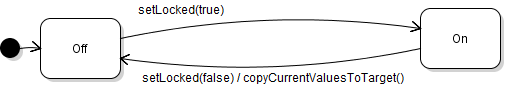
\includegraphics[width=0.75\linewidth]{assets/chpt_impl/sw/AxisManager_onoff}
\end{figure}

\section{Grasp Synergies}
The grasp synergy approach is implemented according to the concepts described in Section \ref{sec:conc:synergy}. The approach are implemented using a gesture page and relative and absolute approach are differentiable by the title of the tabbed page selector, apart from that, the pages look the same.

\subsection{Gesture Parsing}

Gesture parsing is separated into multiple classes. The \textit{GestureParser} class accepts touch events redirected to it by the \textit{GestureView}s on the pages for gesture control. It has a method 
\begin{lstlisting}
public void handleTouchEvent(MotionEvent e);
\end{lstlisting}
which is called from within the \textit{onTouchEvent()} handler of the user interface element. The \textit{GestureParser} is otherwise independent from the user interface element it is invoked by. When a new pointer is encountered, it adds it to a gesture it fits to which is already present on the screen or -- if the pointer is too far away from any existent gesture -- creates a new gesture. If a pointer is removed from the screen, it is also deleted from the gesture it was assigned to. If no pointers are left within the gesture, it is also removed. If an event is received stating a pointer has moved, the pointer location is updated in memory. Upon all of the described actions, the observers of the \textit{GestureParser} are notified. These observers implement the \textit{GestureObserver} interface, which is shown in Listing \ref{lst:impl:gestobs}. It gives the \textit{GestureParser} to notify observers about the addition or removal of a gesture, as well as the case on which a pointer of the gesture has changed its position. 

\begin{lstlisting}[caption={The GestureObserver interface}, label=lst:impl:gestobs]
public interface GestureObserver {
	void onGestureAdd(Gesture g);
	void onGestureRemove(Gesture g);
	void onGestureChanged(Gesture g);
}
\end{lstlisting}

If the pointer count of a gesture changes, the \textit{GestureParser} calls the \textit{onGestureRemove()} method of observers, and then the \textit{onGestureAdd()} method. Both with the same \textit{Gesture} object.

When a gesture is added or its pointer count changes, it is marked as \textit{locked} by the \textit{GestureParser} for the duration of one second. This indicates to dependent classes, that the gesture is new and the data should not yet be used for any control purposes, as the user might still adjust finger positions. This also takes care of the fact that, to add a multi-pointer gesture, the android system calls different events for each pointer subsequently, meaning that to the software it looks as if a one-pointer gesture was added, then a two-pointer gesture and then a three-pointer gesture, if 3 fingers were laid on the touchscreen. By ignoring gesture input for the first second of a new gesture, the user should have put all fingers onto the screen and can then control the application. Having input by an unwanted gesture may cause unexpected behaviour. In the following the functionality of the three main material classes \textit{Location}, \textit{Pointer} and \textit{Gesture} is explained.

\subsubsection{The Location class}

The \textit{Location} class represents a two-dimensional vector within the program. It has two coordinates, $x$ and $y$, which can be accessed by getter methods. It also offers basic functionality to work with vectors, including addition, subtraction, multiplication with scalars and the scalar-product. All functionality is implemented as expected by common sense. When a mathematical operation is performed using two \textit{Location} objects, the result is returned as a new one, as a \textit{Location} is immutable once it is created.

\begin{lstlisting}[caption={The public interface of the Location class}, label=lst:impl:location]
public class Location {
	public Location(float x, float y);
	
	public float getX();
	public float getY();
	
	public Location add(Location loc);
	public Location substract(Location loc);
	public Location multiply(float c);
	public Location divide(float c);
	
	public double scalarProduct(Location loc);
	
	public double getVectorLength();
	public double distanceTo(Location loc);
	public double getAngleTo(Location loc);
	public Location getTurned(double angleRad);
	public boolean isSame(Location l2);
}
\end{lstlisting}

As visible in Listing \ref{lst:impl:location} multiple advanced operations are also available on \textit{Locations}. \textit{getVectorLength()} returns the length of the vector calculated using the Pythagorean theorem. \textit{getDistanceTo()} is implemented very similar, as it basically calculates the length of the differential vector between the \textit{Location} it is invoked on and the passed second \textit{Location}. Although this could be done by one \textit{substract()} operation and then performing \textit{getVectorLength()} on the result the calculation is directly implemented here for performance reasons.

\begin{lstlisting}[caption={Implementation of getVectorLength() and getDistanceTo()},label=lst:impl:location_length]
public double getVectorLength() {
	return Math.sqrt(Math.pow(x, 2) + Math.pow(y, 2));
}

public double distanceTo(Location loc) {
	return (float)Math.sqrt(Math.pow(loc.x - this.x, 2) + Math.pow(loc.y - this.y, 2));
}
\end{lstlisting}

\textit{getAngleTo()} returns the angle between the \textit{Location} it is invoked on and the one passed as a parameter. Please note that this represents the calculation as defined in Equation \ref{eq:conc:orientation} implemented for arbitrary vectors. This means that the output of this method ranges from $-\pi$ to $\pi$, with positive angles meaning a clockwise rotation from the invoked \textit{Location} to the one passed as a parameter. The reader if referred to Listing \ref{lst:impl:angles} for the implementation of \textit{getAngleTo()}. In Line 4 the determinant of the two combined vectors is calculated and the result is multiplied with $-1$ if the determinant is negative. This could've been written shorter, but for better readability this format was chosen.

\begin{lstlisting}[caption={Implementation of getAngleTo()},label=lst:impl:angles]
public double getAngleTo(Location loc) {
	double val = Math.acos(scalarProduct(loc) / (getVectorLength() * loc.getVectorLength()));
	
	if(x * loc.getY() - y * loc.getX() < 0) {
		val *= -1;
	}

	return val;
}
\end{lstlisting}

Lastly, \textit{getTurned()} returns the current \textit{Location} rotated by an angle of \textit{angleRad}. The angle may range from $-\pi$ to $\pi$, with positive angles meaning a clockwise rotation. \textit{isSame()} is a numerical comparison of the two vectors. Note that floating point numbers are compared here, on which equality comparisons are problematic. This function is used to check for exactly the same values, meaning probably the same location objects.

\subsubsection{The Pointer class}

Pointers are the contents of \textit{Gestures}. They contain of a \textit{Location}, representing their coordinates on the touch-screen and an id, which is their touch-pointer-id as assigned by the Android operating system. This class was basically introduced to semantically separate the pointer id from the location. The id is needed to identify a pointer within the motion event raised by the operating system. A method is provided to update the location of a pointer, in which a new \textit{Location} object is created.
\begin{lstlisting}[caption={The Pointer class}]
public class Pointer {
	public Pointer(int id, float x, float y);

	public int getId();

	public Location getLocation();
	public void setLocation(float x, float y);
}
\end{lstlisting}

\subsubsection{The Gesture class}

The \textit{Gesture} class represents a gesture as defined in Section \ref{sec:conc:gestures}. It is basically a set of \textit{Pointer}s with a set of properties. Its public interface is denoted in Listing \ref{lst:impl:gestureclass}.

\begin{lstlisting}[caption={Public interface of the Gesture class},label=lst:impl:gestureclass]
public class Gesture {
	public boolean isLocked();
	public void setLocked(boolean locked);
	
	public void addPointer(Pointer p);
	public void removePointer(Pointer p);
	public int getPointerCount();
	
	public boolean catchesPointer(Pointer p);
	public float getCatchRadius();
	public float getDistanceToCenter(Pointer p);
	
	public Location getCenter();
	public float getSize();
	public double getOrientation();
}
\end{lstlisting}

The first two methods set and query the \textit{locked} state of a gesture, followed by three methods to add and remove pointers, as well as querying the number of currently available pointers in a gesture. Whenever a pointer is added or removed to or from a gesture, the \textit{thumb pointer} is evaluated according to the rules defined in Section \ref{sec:conc:gestures}.
\textit{catchesPointer()} determines whether a new \textit{Pointer} can be added to the gesture. This is done by checking whether the \textit{Pointer}  is within a distance of $2.5$x the size of the gesture around its center. If only one pointer is present in a gesture no size is available. In that case, a size of 1200 is taken as the \textit{catch radius}. \textit{getCenter()}, \textit{getSize()} and \textit{getOrientation()} represent $c(G)$, $s(G)$ and $o(G)$ as defined in section \ref{sec:conc:gestures}.

\subsection{Arm Control}
\label{sec:impl:armcontrol}
\subsubsection{The PointInSpace class}

The \textit{PointInSpace} class implements functionality as a vector in three dimensions, offering basic operations like adding other \textit{PointInSpace} instances and multiplying with scalars. It is not as elaborated as the \textit{Location} class, but extending the functionality according to \textit{Location} if needed could easily be done.

\begin{lstlisting}[caption={The public interface of PointInSpace}]
public class PointInSpace {
	public PointInSpace(double x, double y, double z);
	
	public double getX();
	public double getY();
	public double getZ();
	
	public PointInSpace add(PointInSpace pw);
	public PointInSpace multiply(double v);
}

\end{lstlisting}

\subsubsection{The CartesianArmManager class}

The functionality to move the arm (or better: The palm of the robotic hand) in Cartesian space is provided by the \textit{CartesianArmManager}. It accepts positions for the palm and manages the querying of the BioIK service asynchronously in the background. Once it received a result from the IK service it forwards it to the \textit{AxisManager} instance. It holds a list of all joints that shall not be affected by the \textit{CartesianArmManager}, i.e. all joints of the Shadow C5 hand, thus placement of the palm only takes place by moving joints belonging to the Kuka robot arm. It also only updates joints in the \textit{AxisManager} that it shall affect, leaving control to all the other joints to different parts of the software.

\begin{lstlisting}[caption={The public interface of CartesianArmManager}, label=lst:impl:cartarm]
public class CartesianArmManager implements ServiceResponseListener<bio_ik_msgs.GetIKResponse> {
	public static final double Y_MIN = -1.2;
	public static final double Y_MAX = -0.8;
	public static final double X_MIN = -0.2;
	public static final double X_MAX = 0.4;
	public static final double Z_MIN = 1.05;
	public static final double Z_MAX = 1.17;
	
	public static final int MAX_AXIS_CHANGE = 15;
	
	public static CartesianArmManager getInstance();
	
	public void setNode(C5LwrNode node);
	
	
	public boolean goHome();
	public boolean movePalm(PointInSpace offset);
	public boolean movePalmTo(PointInSpace position);
	
	public PointInSpace getPosition();
	
	public void stop();
}
\end{lstlisting}

\begin{wrapfigure}[20]{R}{0.5\linewidth}
	\caption{\label{fig:impl:cartarmstate}State diagram for the CartesianArmManager update loop}
	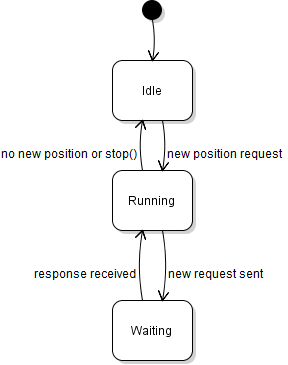
\includegraphics[width=\linewidth]{assets/chpt_impl/sw/CartesianArmManager_loop}
\end{wrapfigure}

Whenever a new target position for the palm is set using \textit{goHome()}, \textit{movePalm()} or \textit{movePalmTo()}, the IK-loop within the \textit{CartesianArmManager} is started. It tries to get solutions from as BioIK service as fast as it can, initiating a new request as soon as one result was received until either no new position was requested or \textit{stop()} was called. Once one of these two cases happen, the loop is stopped and restarted only when a new position is set. Whenever the loop starts a new request, it uses the last set value as target value, values set in between two requests are omitted. Figure \ref{fig:impl:cartarmstate} gives an overview about this process in form of a state diagram.

When a result is returned by the BioIK service it has to go through multiple checks before it is sent to the robot. First, if the \textit{error\_code} field has another value than $0$, the BioIK solver could not find any solution for the queried robot pose, in this case, the \textit{CartesianArmManager} sends the same request to the BioIK service again so it tries to find another solution again. If the \textit{error\_code} field is $0$, the joint angles from the solution are compared to the currently measured state of the robot. When one joint is changed by more than 15 degrees, the solution is rejected as unsafe and a new solution for the same request is queried at the BioIK service. This is done to prevent big movements in joint space, possibly causing unwanted and uncontrollable movements of the robot, potentially causing damage to the robot or its environment. The check for high distances in joint space can be bypassed, which is used when letting the robot go into home position, as this specific position most probably has a bigger distance to the state before than allowed by the check. This means that \textbf{when going to the home position, the user has to watch the robot and has to use caution when using this functionality.} Whenever unwanted movement is observed the user can lift the finger off the safety interlock button to immediately stop any robot movement. As an additional precautionary measure, a hardware emergency switch should be within reach of the operator. When the above checks pass, the joint angled of the arm returned by the BioIK service are written to the \textit{AxisManager} which then sends them to the robot over ROS.

The functionality of the three methods to set new target value is in particular:
\begin{itemize}
	\item \textit{goHome()} sets the target position of the palm to a fixed position which is known to be safely reachable. In this case, it's $p_{home} = \vecthr{0}{y_{min}}{z_{max}}$, which is a position located directly in front of the robot at the border of the table.
	\item \textit{movePalm()} moves the current target position of the palm by \textit{offset} (by adding it to the position returned by \textit{getPosition()}).
	\item \textit{movePalmTo()} overwrites the target position by \textit{position}.
\end{itemize}



\subsection{Absolute control}

\subsection{Relative control}

\section{Direct Finger Positioning}
\label{sec:impl:dfmt}

\section{Performance}

\subsection{Application}

\subsection{BioIK Service}

\chapter{Evaluation}
\label{chap:eval}

\section{Usability}

First tests and trials have shown that the different approaches yield different results regarding simplicity, manoeuvrability and usability. No formal tests and studies have been conducted by now, the following experiences are subjective and by far not representative.

Controlling the hand grasps using the grasp synergy approaches works decently good. The absolute version seems to give the user a little better and more direct control about what is actually happening with the hand and thus more dexterity in the grasp operations than the relative approach. Controlling the arm in both approaches, however, is fairly inaccurate. 
In the absolute approach, inaccuracies derive from the small screen size which is mapped to a relatively large workspace. In the relative approach the arm can be controlled more precisely, but the activation time of one second for a new gesture is significantly affecting the workflow. Whenever the gesture is lifted and moved to the other end of the screen to perform another relative movement of the arm, the operator has to wait one second.
In both approaches, however, the arm does not remain at one stable position when the control gesture is stationary. This results in a noticeable jitter of the arm. The reason for this seems to be the BioIK solver returning different solutions for the same pose. As long as the gesture is active on the screen, new solutions are queried by the application in an endless loop, since the position of the pointers change very little. These changes are in the second to fourth decimal digit of the value of the amplitude, however the BioIK solver returns a new -- and different -- solution for the same position. This effect was dramatically reduced once the \textit{MinimalDisplacementGoals} were added to the request messages, but are still noticeable. Additionally, finding solutions with the \textit{MinimalDisplacementGoal} active in the request takes significantly longer (about factor two, see Section \ref{sec:eval:ikservice}).  These small movements made precise control and positioning of the hand difficult. One possible solution could be to monitor the movement of a gesture and only calculate new values when movements above a certain threshold (e.g. 10 pixels) occur.

In the direct fingertip mapping, these jitters were even more significant, as the position of the fingertips were to be mapped to positions in space with high dexterity. However, because of the jitter occurring within the BioIK solutions, it is very hard to precisely grasp objects. Again, adding the \textit{MinimumDisplacementGoal} reduced this effect significantly, but slowed down the (already slow) solution finding of BioIK even more.

\section{Performance}

As performance issues occurred during first tests, a small look into where these issues arise shall be given.

\subsection{Application}

The overall performance of the application seems sufficient. No significant lags in response times of the user interface were noticeable. All off-line calculations like calculating joint angles from grasp synergies or fingertip positions in three dimensions do not take any significant processing power. While using the application without any inverse kinematic involved, the CPU load was measured well below 5\%. Nonetheless, the device gets significantly warm after a period of usage and the battery power drains perceptibly faster compared to everyday use. 

No further effort was done to find out the reason for the warmth and battery drain as it did not directly affect development, but a good assumption might be that the ROS data exchange induces a constant load onto the WiFi chipset of the tablet computer. Joint states are received at about 100 Hz, updates are sent at 10 Hz. Additionally, every BioIK service call issues some wireless communication. This leads to a lot of small packets being sent over the wireless network, resulting in a constant workload preventing the chipset from being put into power saving modes.

\subsection{BioIK Service}
\label{sec:eval:ikservice}

\begin{figure}
	\caption{\label{fig:eval:1000ms}Measurements for 1000ms}
	\begin{center}
		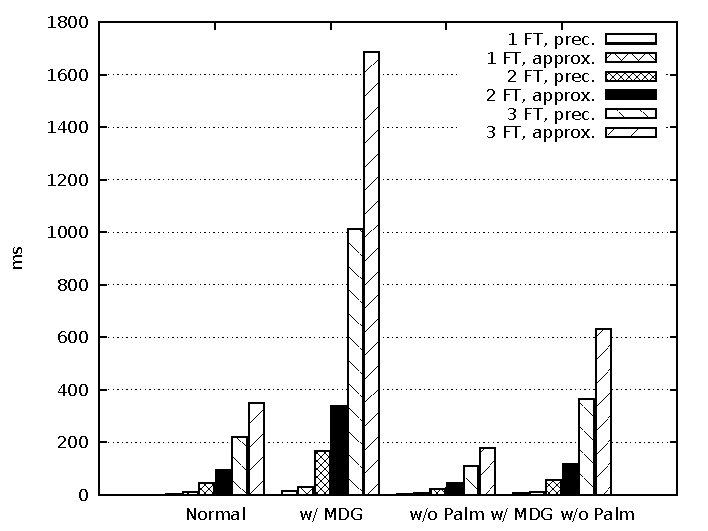
\includegraphics{assets/chpt_eval/1000ms.pdf}
	\end{center}
\end{figure}


It was observed during tests that getting a result from the BioIK service takes significant amounts of time during arm movements controlled by touch gestures and even more time in the direct fingertip mapping mode. In the grasp synergy approaches, an IK request took about 200-300 ms from sending the request until the \textit{onSuccess()} callback was called in the application. This is a frequency of about 5Hz, which is lower than expected but still enough for a relatively precise positioning of the arm.

In the direct fingertip mapping approach however, response times varied depending on the number of fingers that were currently mapped, from approx. 600ms when using one finger to about 1.6 seconds with three fingers on the screen. Update frequencies of significantly less than 1 Hz are very disturbing and prevent the application from being used in the desired manner.

Additionally it is observable that when the BioIK service is called, the user interface freezes until a response is processed, resulting in a very juddery user experience. Multiple factors can take effect here:
\begin{itemize}
	\item The rosjava/rosandroid implementation of service calls is faulty. The freezing user interface is an indication for the service calls not being implemented asynchronously as one would think, since a call is initiated with a service response handler which is called when the result was received.
	\item The BioIK service is very slow or has unexpected behaviours.
\end{itemize}

Since debugging of foreign code can be very time-consuming, especially in projects of the size of rosjava and rosandroid, first measurements were done concerning the performance of BioIK. A pose of the robot was chosen which was once returned by the BioIK service, so it' iss known that a solution exists. Then, the following cases were measured:
\begin{itemize}
	\item 1, 2 and 3 fingertips with \textit{approximate = false}.
	\item 1, 2 and 3 fingertips with \textit{approximate = true}.
\end{itemize}

for the following cases:
\begin{itemize}
	\item With \textit{OrientationGoal} for the palm, without \textit{MinimumDisplacementGoal}.
	\item Without \textit{OrientationGoal} for the palm, without \textit{MinimumDisplacementGoal}.
	\item With \textit{OrientationGoal} for the palm, with \textit{MinimumDisplacementGoal}.
	\item Without \textit{OrientationGoal} for the palm, with \textit{MinimumDisplacementGoal}.
\end{itemize}

Every test request was executed 200 times, as a result the mean execution time of all calls was taken. The aim was to find out what affects execution time of the BioIK service the most, the suspected properties were the \textit{MinimumDisplacementGoal}, the additional \textit{OrientationGoal} for the palm and the \textit{approximate} property of the IK request. Measurements were initially done with a timeout of one second passed to the BioIK solver. A plot of the measurements can be reviewed in Figure \ref{fig:eval:1000ms}. Three interesting aspects are visible on the first sight:
\begin{itemize}
	\item If the request is marked with \textit{approximate = true}, the solver takes about twice the time as if a precise solution is requested.
	\item The \textit{MinimumDisplacementGoal} seems to have a huge effect on execution time, multiplying the time by a factor of about 4-5.
	\item The time needed by the solver is highly dependent on the number of fingertips included in the request. 
\end{itemize}

\begin{figure}
	\caption{\label{fig:eval:10ms}Measurements for 10ms}
	\begin{center}
		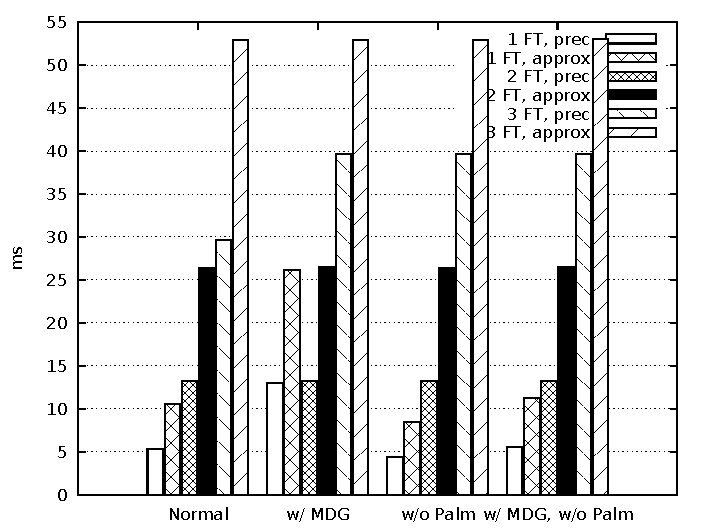
\includegraphics{assets/chpt_eval/10ms.pdf}
	\end{center}
\end{figure}

All tests were repeated setting the \textit{timeout} for the request to 10 ms. The test results are represented in Figure \ref{fig:eval:10ms}. Surprisingly this rendered all measurements completely different. Execution times are nearly constant for every fingertip configuration, the dependency seems to be exponential. The only real difference visible is the measurement of one fingertip with \textit{OrientationGoal} for the Palm and with \textit{MinimumDisplacementGoal}, which is about factor three bigger than without the \textit{MinimumDisplacementGoal}. Most importantly, the maximum times of about 55ms were about two orders of magnitude smaller than the maximum values measured with a timeout of one second. The execution time of the BioIK solver seems to be dependent on the passed timeout, using more time when the timeout is bigger. This assumption was confirmed by \citeauthor{Ruppel17}\cite{Ruppel17} who states that the BioIK solver \textbf{can} return a result before the timeout is exceeded, but does not necessarily do so.

As a consequence, a time-out of 10ms was set for the BioIK service calls within the Android application. The results, again, were surprising, as no significant improvement was observed. The only difference then was that the BioIK solver returned an error code indicating no solution was found, increasing the timeout up to 500ms rendered the DFTM approach usable again, but still with response times of 1.2 to 1.6 seconds. At the time of writing open questions remain. It is yet to be found out why the service calls take such a long time in rosjava/rosandroid, rendering the user interface frozen with the response time not significantly impacted by the timeout set in the request. As the measurements suggest, however, the main issue should probably be searched for within the rosjava and rosandroid implementations, as solving times were found reasonable when calling the BioIK service isolated.

\section{Possible User Studies}

With user studies, one could find out how well the different approaches implemented here work with untrained and trained test persons. Data can be recorded either objectively by measuring times and judging how successful the execution of a task has been or subjectively, by asking the user about how difficult the task was. A famous, standardized questionnaire is the NASA TLX (Task Load Index) test\cite{Hart1988}. It yields a good insight of how stressful a task was for the user. Apart from these standardized tests, a domain-specific test should be developed to get data about the actual environment that shall be evaluated.

Each test person should perform multiple tasks with a rising level of difficulty. For example:
\begin{itemize}
	\item Grasp an object and release it.
	\item Grasp an object, move it to another place and release it.
	\item Grasp an object, put it into a box placed nearby.
\end{itemize}
These tasks can then be performed for both multiple objects (balls, cylinders, cuboids) of different materials (sponge, wood, rubber) and the three different approaches. Each task shall be completed multiple times, while the time needed to complete the task is measured. This gives an insight in how fast a specific task can be trained. Additionally, after the task was executed multiple times by one user, he shall be queried for how difficult he thinks the task was, how much help he needed and how intuitive he thinks the control was. The test supervisor shall also note how much help he had to give to the test person to give an insight on how different perception was. 

From the data raised during these studies a conclusion can be made which approach is probably the best to grasp a variety of objects, which is the easiest to learn, which one is the most intuitive and which one causes the least stress on the operator. These results could then be used in further development and improvement of tele-manipulation methods using a dexterous robotic hand and a robot arm, combined to a robot system with a high number of degrees-of-freedom.

\chapter{Conclusion}
\label{chap:concl}

The application that was developed within this thesis shows the principle possibilities to control a robot with many DOF using a generic end-user multitouch device running the Android operating system. Having implemented multiple approaches gave an insight into different possibilities to perform tele-operation of a robot and  tele-manipulating its environment. While the gesture parsing functionality developed gives a generic method to explore the properties of a simple multi-pointer gesture, which may be used for other purposes as well, the direct fingertip mapping approach showed that mapping of pointers in two dimensions into a three-dimensional space is a task that can be performed with basic maths operations.

First tests were done using the given set-up. Besides some hardware-related issues (like missing air pressure) the functionality mostly worked as expected, only the jitters of the arm in all approaches were a significant drawback, which is what future work should probably put some effort into. Of course, more tests and studies have to be conducted and parameters of the different approaches (especially the relative grasp synergy approach) have to be optimized.

\section{Outlook}

Future work could concentrate on several things. First, the occurred performance and jittering issues should be reviewed. The performance issues can probably be resolved by looking into the rosjava and rosandroid implementations, where at least a factor of two is situated. After that, a look into the jittering of BioIK solutions would be an interesting thing to look into, as precise grasping actions depend on a stable and dexterous positioning of effectors. If these problems are solved, statistically significant user studies should be conducted to deeply evaluate the usability of the different approaches and give suggestions on improving them.

In the end, the application is designed in a way that should make it easy to implement more methods of controlling a robot as they come up and are researched, using the existing framework of \textit{AxisManager} and \textit{C5LwrNode} and the given user interface structure.

\cleardoublepage

%% VERZEICHNISSE (Abbildungen, Tabellen)
% Literatur 

\printbibliography

\listoffigures

\listoftables

\lstlistoflistings

\cleardoublepage

% ERKLÄRUNG
\chapter*{Eidesstattliche Versicherung}
\thispagestyle{empty}
\addcontentsline{toc}{chapter}{Eidesstattliche Versicherung}

Hiermit versichere ich an Eides statt, dass ich die vorliegende Arbeit im
Bachelorstudiengang Informatik selbstständig verfasst und keine anderen als die
angegebenen Hilfsmittel -- insbesondere keine im Quellenverzeichnis nicht
benannten Internet-Quellen -- benutzt habe. Alle Stellen, die wörtlich oder
sinngemäß aus Veröffentlichungen entnommen wurden, sind als solche kenntlich
gemacht.
Ich versichere weiterhin, dass ich die Arbeit vorher nicht in einem anderen Prüfungsverfahren eingereicht habe und die eingereichte schriftliche Fassung der auf dem elektronischen Speichermedium entspricht.

\noindent Ich bin mit einer Einstellung in den Bestand der Bibliothek des Fachbereiches einverstanden.

\vspace{2cm} 

\noindent Reinfeld, den \uline{~~~~~~~~~~~~~~~~~~~~}~~~~~Unterschrift: \uline{~~~~~~~~~~~~~~~~~~~~~~~~~~~~~~~~~~~~~~~~~~~~~~~~~~} 

    
\end{document}